\ifdefined\included
\else
\documentclass[a4paper,11pt,twoside]{StyleThese}
\usepackage{amsmath,amssymb}             % AMS Math
\usepackage[french]{babel}
\usepackage[utf8]{inputenc}
\usepackage[T1]{fontenc}
\usepackage{tabularx}
%\usepackage{tabular}
\usepackage{multirow}


\usepackage[tight,footnotesize]{subfigure}
\usepackage{algorithm} %To allow algorithm environment
\usepackage{algpseudocode} %Provides algorithmic environment

\usepackage{hhline}
\usepackage[left=1.5in,right=1.3in,top=1.1in,bottom=1.1in,includefoot,includehead,headheight=13.6pt]{geometry}
\renewcommand{\baselinestretch}{1.05}

% Table of contents for each chapter

\usepackage[nottoc, notlof, notlot]{tocbibind}
\usepackage[french]{minitoc}
\setcounter{minitocdepth}{2}
\mtcindent=15pt
% Use \minitoc where to put a table of contents

\usepackage{aecompl}

% Glossary / list of abbreviations

\usepackage[intoc]{nomencl}
\renewcommand{\nomname}{Liste des Abréviations}

\makenomenclature

% My pdf code

\usepackage{ifpdf}

\ifpdf
  \usepackage[pdftex]{graphicx}
  \DeclareGraphicsExtensions{.jpg}
  \usepackage[a4paper,pagebackref,hyperindex=true]{hyperref}
  \usepackage{tikz}
  \usetikzlibrary{arrows,shapes,calc}
\else
  \usepackage{graphicx}
  \DeclareGraphicsExtensions{.ps,.eps}
  \usepackage[a4paper,dvipdfm,pagebackref,hyperindex=true]{hyperref}
\fi

\graphicspath{{.}{images/}}

%nicer backref links
\renewcommand*{\backref}[1]{}
\renewcommand*{\backrefalt}[4]{%
\ifcase #1 %
(Non cité.)%
\or
(Cité en page~#2.)%
\else
(Cité en pages~#2.)%
\fi}
\renewcommand*{\backrefsep}{, }
\renewcommand*{\backreftwosep}{ et~}
\renewcommand*{\backreflastsep}{ et~}

% Links in pdf
\usepackage{color}
\definecolor{linkcol}{rgb}{0,0,0.4} 
\definecolor{citecol}{rgb}{0.5,0,0} 
\definecolor{linkcol}{rgb}{0,0,0} 
\definecolor{citecol}{rgb}{0,0,0}
% Change this to change the informations included in the pdf file

\hypersetup
{
bookmarksopen=true,
pdftitle="Évaluation de la sécurité des équipements grand public connectés à Internet",
pdfauthor="Yann BACHY", %auteur du document
pdfsubject="Thèse", %sujet du document
%pdftoolbar=false, %barre d'outils non visible
pdfmenubar=true, %barre de menu visible
pdfhighlight=/O, %effet d'un clic sur un lien hypertexte
colorlinks=true, %couleurs sur les liens hypertextes
pdfpagemode=None, %aucun mode de page
pdfpagelayout=SinglePage, %ouverture en simple page
pdffitwindow=true, %pages ouvertes entierement dans toute la fenetre
linkcolor=linkcol, %couleur des liens hypertextes internes
citecolor=citecol, %couleur des liens pour les citations
urlcolor=linkcol %couleur des liens pour les url
}

% definitions.
% -------------------

\setcounter{secnumdepth}{3}
\setcounter{tocdepth}{2}

% Some useful commands and shortcut for maths:  partial derivative and stuff

\newcommand{\pd}[2]{\frac{\partial #1}{\partial #2}}
\def\abs{\operatorname{abs}}
\def\argmax{\operatornamewithlimits{arg\,max}}
\def\argmin{\operatornamewithlimits{arg\,min}}
\def\diag{\operatorname{Diag}}
\newcommand{\eqRef}[1]{(\ref{#1})}

\usepackage{rotating}                    % Sideways of figures & tables
%\usepackage{bibunits}
%\usepackage[sectionbib]{chapterbib}          % Cross-reference package (Natural BiB)
%\usepackage{natbib}                  % Put References at the end of each chapter
                                         % Do not put 'sectionbib' option here.
                                         % Sectionbib option in 'natbib' will do.
\usepackage{fancyhdr}                    % Fancy Header and Footer

% \usepackage{txfonts}                     % Public Times New Roman text & math font
  
%%% Fancy Header %%%%%%%%%%%%%%%%%%%%%%%%%%%%%%%%%%%%%%%%%%%%%%%%%%%%%%%%%%%%%%%%%%
% Fancy Header Style Options

\pagestyle{fancy}                       % Sets fancy header and footer
\fancyfoot{}                            % Delete current footer settings

%\renewcommand{\chaptermark}[1]{         % Lower Case Chapter marker style
%  \markboth{\chaptername\ \thechapter.\ #1}}{}} %

%\renewcommand{\sectionmark}[1]{         % Lower case Section marker style
%  \markright{\thesection.\ #1}}         %

\fancyhead[LE,RO]{\bfseries\thepage}    % Page number (boldface) in left on even
% pages and right on odd pages
\fancyhead[RE]{\bfseries\nouppercase{\leftmark}}      % Chapter in the right on even pages
\fancyhead[LO]{\bfseries\nouppercase{\rightmark}}     % Section in the left on odd pages

\let\headruleORIG\headrule
\renewcommand{\headrule}{\color{black} \headruleORIG}
\renewcommand{\headrulewidth}{1.0pt}
\usepackage{colortbl}
\arrayrulecolor{black}

\fancypagestyle{plain}{
  \fancyhead{}
  \fancyfoot{}
  \renewcommand{\headrulewidth}{0pt}
}

%\usepackage{MyAlgorithm}
%\usepackage[noend]{MyAlgorithmic}
\usepackage[ED=MITT - STICIA, Ets=INP]{tlsflyleaf}
%%% Clear Header %%%%%%%%%%%%%%%%%%%%%%%%%%%%%%%%%%%%%%%%%%%%%%%%%%%%%%%%%%%%%%%%%%
% Clear Header Style on the Last Empty Odd pages
\makeatletter

\def\cleardoublepage{\clearpage\if@twoside \ifodd\c@page\else%
  \hbox{}%
  \thispagestyle{empty}%              % Empty header styles
  \newpage%
  \if@twocolumn\hbox{}\newpage\fi\fi\fi}

\makeatother
 
%%%%%%%%%%%%%%%%%%%%%%%%%%%%%%%%%%%%%%%%%%%%%%%%%%%%%%%%%%%%%%%%%%%%%%%%%%%%%%% 
% Prints your review date and 'Draft Version' (From Josullvn, CS, CMU)
\newcommand{\reviewtimetoday}[2]{\special{!userdict begin
    /bop-hook{gsave 20 710 translate 45 rotate 0.8 setgray
      /Times-Roman findfont 12 scalefont setfont 0 0   moveto (#1) show
      0 -12 moveto (#2) show grestore}def end}}
% You can turn on or off this option.
% \reviewtimetoday{\today}{Draft Version}
%%%%%%%%%%%%%%%%%%%%%%%%%%%%%%%%%%%%%%%%%%%%%%%%%%%%%%%%%%%%%%%%%%%%%%%%%%%%%%% 

\newenvironment{maxime}[1]
{
\vspace*{0cm}
\hfill
\begin{minipage}{0.5\textwidth}%
%\rule[0.5ex]{\textwidth}{0.1mm}\\%
\hrulefill $\:$ {\bf #1}\\
%\vspace*{-0.25cm}
\it 
}%
{%

\hrulefill
\vspace*{0.5cm}%
\end{minipage}
}

\let\minitocORIG\minitoc
\renewcommand{\minitoc}{\minitocORIG \vspace{1.5em}}

\usepackage{multirow}
%\usepackage{slashbox}

\newenvironment{bulletList}%
{ \begin{list}%
	{$\bullet$}%
	{\setlength{\labelwidth}{25pt}%
	 \setlength{\leftmargin}{30pt}%
	 \setlength{\itemsep}{\parsep}}}%
{ \end{list} }

\newtheorem{definition}{Définition}
\renewcommand{\epsilon}{\varepsilon}

% centered page environment

\newenvironment{vcenterpage}
{\newpage\vspace*{\fill}\thispagestyle{empty}\renewcommand{\headrulewidth}{0pt}}
{\vspace*{\fill}}

\usepackage{tablefootnote}
\sloppy
\begin{document}
\setcounter{chapter}{1} %% Numéro du chapitre précédent ;)
\dominitoc
\faketableofcontents
\fi

\chapter{Construction et Maintien de l'État du Monde}
\label{chapter1}
\minitoc


\section{Contexte}
\subsection{Défis à relever}
Le robot est un système pouvant percevoir, comprendre et agir sur son environnement. Comprendre son environnement suppose de pouvoir raisonner sur les données de perception afin d'en extraire des données de plus haut niveau d'abstraction, permettant d'avoir une estimation de la situation et ainsi de prendre les décisions adéquates pour accomplir la tâche qui lui incombe. C'est la célèbre boucle perception-décision-action.

Avec le progrès récent de la robotique, les robots commencent à arriver dans les usines pour travailler aux côtés d'humains, ainsi que dans les foyers comme robot d'assistance. Adapter les capacités de raisonnements du robot à ce nouveau monde, qui est par définition configuré pour l'homme, représente un défi pour la recherche. Cet environnement humain est composé
d'éléments statiques tel que les murs, d'éléments pouvant évoluer au cours d'une interaction (déplacement, remplissage, activation...) que nous appellerons les objets, et enfin d'éléments pouvant se mouvoir, agir sur les objets, et interagir entre eux que nous appellerons les agents. Ces agents peuvent être robotiques ou humains.
Pour pouvoir agir dans un environnement humain, le robot doit donc pouvoir percevoir tous ces éléments énumérés précédemment et en extraire une représentation symbolique afin de décrire au mieux la situation et permettre à la couche décisionnelle d'agir de façon appropriée.


\subsection{Évaluation de la situation}
\label{sec:evaSit}


Le concept de "connaissance de la situation" (Situation Awareness) a été identifié d'après Gilson \cite{gilson1995} durant la première guerre mondiale par Oswald Boelke qui a réalisé "l'importance d'obtenir une connaissance de l'ennemi avant que l'ennemi n'obtienne une connaissance similaire, et conçu des procédés pour y parvenir". Le terme de Situation Awareness est couramment utilisé dans le domaine de l'Interaction Homme-Machine. Parmi les scientifiques ayant étudié ce principe, Mica Endsley en a énoncé une définition générale. Elle définit la connaissance de la situation comme étant "la perception d'éléments de l'environnement dans un volume de temps et d'espace, la compréhension de leur signification et la projection de leur état dans un future proche" \cite{endsley2000}.
Le chapitre 7, "Situation Awareness" du livre \cite{pew1998modeling} présente une discussion et une étude sur les différentes définitions (données dans divers articles tel que \cite{stiffler1988graduate,noble1989application,fracker1988theory}...) et systèmes pour la connaissance de la situation. Dans l'article \cite{stanton2001situational}, la connaissance de la situation est abordée du point de vue de la sécurité. L'article présente et discute trois théories de la connaissance de la situation: le modèle en trois niveau d'Ensley \cite{endsley1995}, l'approche basée sur les sous-systèmes interactifs \cite{bedny1999theory} et le cycle perceptuel  \cite{smith1995situation}.

\begin{figure}[ht!]
 \centering
  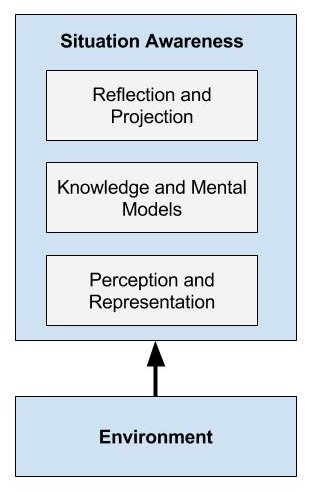
\includegraphics[width=0.49\linewidth]{./img/ensley.jpg} 
  \caption {Schéma présentant le modèle en trois niveaux pour la connaissance de la situation présentée par Ensley.}
  \label{fig:ensley}
\end{figure}

Nous détaillons ici les trois niveaux d'Ensley.
\begin{itemize}
\item Premier niveau: perception des éléments de l'environnement. Ce niveau est l'identification des
éléments ou événements clés qui, en les combinant servent à définir la situation.
Ce premier niveau marque sémantiquement les éléments important de la situation pour
les niveaux d'abstraction supérieure dans les processus suivants.
\item Deuxième niveau: compréhension de la situation courante. La compréhension provient de 
la combinaison des éléments du premier niveau pour avoir une représentation plus globale. Ce niveau permet de
définir l'état courant en des termes pertinents qui permettent la prise de 
décision et d'entreprendre d'agir sur l'environnement.
\item Troisième niveau: prédiction des états futurs. Ce niveau est la projection de la situation courante vers le futur, dans l'environnement, afin d'essayer de prédire l'évolution de la situation. La précision de la prédiction dépend largement de la précision des deux niveaux inférieurs de connaissance de la situation. L'anticipation du futur projeté permet à l'agent décisionnel (l'opérateur ou le superviseur) d'avoir le temps de résoudre certains problèmes avant qu'ils n'arrivent et de mettre en place un plan d'action pour atteindre l'objectif.
\end{itemize}
Cette composition est résumée à la figure \ref{fig:ensley}.

Dans le cas de systèmes en évolution et d'environnements dynamiques, le processus permettant d'acquérir et de maintenir la connaissance de la situation est appelé évaluation de la situation (situation assessment). Endsley explique dans \cite{endsley1995} que "la connaissance de la situation incorpore la compréhension d'un opérateur sur la situation globale, formant ainsi la base pour la prise de décision". Les processus d'évaluation de la situation sont donc fortement liés aux processus de prise de décision (qui constituent la supervision dans un système robotique).
L'une des principales préoccupations pour l'Interaction Homme-Machine est de concevoir des interfaces utilisateurs qui permettent à un opérateur d'acquérir la connaissance de la situation de façon optimale afin qu'il puisse décider quelle décision prendre.

De la même manière, en robotique, le robot a besoin de décider quelle action entreprendre et quand agir sur son environnement. Pour prendre ce genre de décisions, la supervision repose sur des processus de plus bas niveau pour obtenir des informations à haut niveau d'abstraction sur l'environnement. Cela implique, pour l'évaluation de la situation, de raisonner sur ce qui entoure le robot à partir des données des capteurs afin de modéliser la configuration de l'environnement physique autour du robot et de produire un ensemble de propriétés concernant les divers éléments. Ceci permet de fournir une représentation symbolique de l'état du monde au superviseur afin de faciliter son raisonnement et sa prise de décision. Pour créer cette représentation symbolique, il est d'abord nécessaire au robot d'avoir une bonne estimation de l'état du monde et d'en avoir une représentation tridimensionnelle en regroupant efficacement les données de perception issues des divers capteurs.

% 3 different ways to perform SA: 
%https://core.ac.uk/download/files/14/334486.pdf

%http://ieeexplore.ieee.org/xpl/login.jsp?tp=&arnumber=1021221&url=http%3A%2F%2Fieeexplore.ieee.org%2Fiel5%2F7951%2F21965%2F01021221.pdf%3Farnumber%3D1021221
%http://www.control.isy.liu.se/student/exjobb/xfiles/3267.pdf
%http://www.sciencedirect.com/science/article/pii/S0378475408000505
%https://www.cse.ust.hk/~qyang/Docs/1998/irene98.pdf
%http://oai.dtic.mil/oai/oai?verb=getRecord&metadataPrefix=html&identifier=ADA309146
%http://ieeexplore.ieee.org/xpl/login.jsp?tp=&arnumber=334802&url=http%3A%2F%2Fieeexplore.ieee.org%2Fiel3%2F2223%2F7874%2F00334802
%http://proceedings.spiedigitallibrary.org/proceeding.aspx?articleid=1286789
%https://books.google.fr/books?hl=fr&lr=&id=WrJGDsjJakcC&oi=fnd&pg=PA3&dq=situation+assessment+intelligent+system&ots=XHaoxqUmGO&sig=2CsheQK-C0F8PLzvKv3Wzjjqejk#v=onepage&q&f=false
%http://pro.sagepub.com/content/32/2/102.short
%http://ieeexplore.ieee.org/xpl/login.jsp?tp=&arnumber=4308574&url=http%3A%2F%2Fieeexplore.ieee.org%2Fxpls%2Fabs_all.jsp%3Farnumber%3D4308574
%http://ieeexplore.ieee.org/xpl/login.jsp?tp=&arnumber=1021218&url=http%3A%2F%2Fieeexplore.ieee.org%2Fxpls%2Fabs_all.jsp%3Farnumber%3D1021218
%http://repository.tudelft.nl/islandora/object/uuid:d90d6170-ad65-4abd-b4cb-c58a0ab09eb5/?collection=research

%With the recent advances in robotics, robots have begun to appear in our daily lives. The world of a robot is now populated with humans with whom it needs to interact. An important challenge for researchers is to adapt the robot's reasoning capabilities to this new world, which is by default shaped for humans. Human-robot interaction requires to equip the robot with explicit reasoning on the human and on its own capacities to achieve its tasks in a collaborative way with a human partner.

%In our concrete context, a robot and one or several human(s) share a physical environment, typically  a workshop or a domestic environment. The environment is composed of static walls and furnitures. What is dynamic is the fact that humans and robot move and manipulate objects.

%The role of SPARK (\textit{SPAtial Reasoning and Knowledge}) component described here in the robot control architecture is to permanently maintain a state of the world in order to provide a basis for the robot to plan, to act, to react and to interact. In addition, SPARK has been designed in order to take into account the following considerations.
%To tackle this challenge, robot's abilities must be enhanced.

%%%%%%%%%%%
\subsection{État de l'art}

Dans le domaine de l'Intelligence Artificielle, plusieurs méthodes ont été développées pour effectuer l'évaluation de la situation. Nous allons brièvement décrire ces différentes méthodes.

\subsubsection{Évaluation de la situation basée sur des règles expertes}
Un système d'évaluation de la situation basé sur des règles (rule-based en Anglais) est un système de connaissance qui repose sur des règles préétablies pour l'inférence et sur une base de faits. L'expertise liée au domaine est directement intégrée au système par la définition des différentes règles spécifiques au domaine d'application. L'état du monde symbolique en découlant est représenté comme un ensemble de faits dans une base de faits.
Généralement, les règles utilisent des données d'environnements (pouvant provenir de calculs sur les données capteurs) ou des faits provenant d'autres règles, et en fonction de certaines conditions logiques, produisent un nouveau fait qui sera ajouté à la base de faits. 
Par exemple, un système météorologique pourrait avoir la règle suivante: \newline
$HIGH\_TEMPERATURE \land NO\_CLOUD \implies GOOD\_WEATHER$. \newline
Dans cet exemple, les propriétés $HIGH\_TEMPERATURE$ et $NO\_CLOUD$ sont issues de capteurs. Si ces deux propriétés sont vraies, le fait $GOOD\_WEATHER$ sera produit et ajouté à la base de faits. Dans le cas d'un système basé sur des règles expertes, cette implication serait directement ajoutée au système par l'expert du domaine (par exemple ici un expert en météorologie). 
Les modules responsables de la production des faits basés sur ces règles sont appelés des raisonneurs.

En identifiant les divers éléments et leurs relations, les règles peuvent être utilisées pour déduire des informations de plus haut niveau correspondant à des faits décrivant des situations particulières. Ceci permet à la partie décisionnelle, c'est à dire l'opérateur pour une Interface Homme-Machine (IHM) ou le superviseur pour un système autonome tel qu'un robot, de baser sa décision sur des faits décrivant la situation de façon pertinente.

Ce type d'approche a été utilisé dans divers domaines, comme par exemple l'évaluation de la situation pour la surveillance côtière \cite{edlund2006rule}, l'évaluation de procédure d'approche pour l'atterrissage d'avion \cite{baron1980procru,milgram1984multi}, le dépannage de voiture ou encore le diagnostic médical \cite{swartout1985rule,miller1982internist}.
L'un des avantages principaux des systèmes basés sur des règles est qu'ils sont relativement simples et naturels dans leur implémentation.
Cependant, l'un des inconvénients de tels systèmes est le manque de modélisation de l'incertitude.
Même si certaines variantes de systèmes basés sur des règles incorporent des valeurs d'incertitudes dans les règles, cette approche implique certaines restrictions et une attention toute particulière lors du développement des règles comme présenté au chapitre 15 du livre \cite{russell2003artificial}.


\subsubsection{Évaluation de la situation basée sur le cas}
%http://www.nap.edu/read/6173/chapter/9#185
%https://www.nada.kth.se/utbildning/grukth/exjobb/rapportlistor/2007/rapporter07/laxhammar_rikard_07046.pdf
%p21
%...

Le raisonnement basé sur le cas (Case-based reasoning en Anglais) est un paradigme dans lequel la connaissance est représentée comme un ensemble de cas individuels qui est utilisé pour raisonner sur de nouvelles situations. Tous les cas partagent une même structure et sont définis par un ensemble de caractéristiques. Lorsqu'un nouveau problème, défini comme le cas recherché, est présenté au système, il est comparé à tous les autres cas de la bibliothèque, et le cas le plus proche est utilisé pour résoudre le nouveau problème. La proximité est définie par une mesure basée sur un sous-ensemble des caractéristiques du cas appelé indice de caractéristiques. Il existe différents types de mesures de similarité: distance Euclidienne, distance d'Hamming, la métrique de la valeur de différence de Stanfill et Waltz (1986)...

En général, le cas le plus proche retrouvé ne correspond pas parfaitement au cas recherché. C'est pourquoi, les systèmes basés sur le cas ont souvent recours à des règles pour adapter le cas retrouvé au cas recherché.
L'un des intérêts d'utiliser le raisonnement basé sur le cas pour l'estimation de la situation et la prise de décision est que cette démarche est proche de celle utilisée par les hommes pour interagir sur leur environnement. Dans le domaine de la théorie de la mémoire humaine, ce cas de connaissance liée à un épisode spécifique est appelé la mémoire épisodique \cite{tulving1972episodic}.

L'approche basée sur le cas peut également être préférable lorsqu'il n'y a pas de modèles valides du domaine. En effet, dans certaines applications l'espace d'états peu être trop vaste pour permettre la construction d'un domaine complet et pertinent. En l'absence de la modélisation du modèle, les solutions basées sur le cas offrent une alternative aux solutions basées sur le modèle.




% disadvantages. Models are condensed summaries of a domain, omitting (i.e., averaging over) details below a certain level. They therefore contain less information (i.e., fewer parameters) and require less storage space and have less computational complexity than case-based approaches. If it is known beforehand that there will never be a need to access details below the model's level of abstraction, models are preferable because of their increased computational efficiency. However, if access to low-level information will be needed, a case-based reasoning approach is preferable.

% We are unaware of any military human behavior representations that employ case-based reasoning models of situation awareness. However, we believe this approach offers considerable potential for the development of general situation awareness models and military situation awareness models in particular, given the military's heavy reliance on case-based training through numerous exercises, the well-known development of military expertise with actual combat experience, and the consistent use of "war stories" or cases by subject matter experts to illustrate general concepts. In addition, the ease with which case-based reasoning or case "learning" can be implemented makes the approach particularly attractive for modeling the effects of human learning. Whether effective case-based reasoning models of situation awareness will be developed for future human behavior representations is still an open research question, but clearly one worth pursuing.


\subsubsection{Évaluation de la situation basée sur des Réseaux Bayésiens}
%https://www.nada.kth.se/utbildning/grukth/exjobb/rapportlistor/2007/rapporter07/laxhammar_rikard_07046.pdf
%http://www.nap.edu/read/6173/chapter/9#186
%TODO check with livre ^

Pour réaliser l'estimation de la situation de façon probabiliste, de nombreux systèmes ont recours à divers
variantes des réseaux Bayésiens (BN pour Bayesian Networks) \cite{bladon2002situation,das2002situation,higgins2005automatic}.
Les réseaux Bayésiens (aussi appelés réseaux de croyance (Belief Networks) ou réseaux de croyance Bayésien (BBN pour Bayesian Belief Networks) sont des structures probabilistes qui permettent un raisonnement cohérent à partir d'informations incertaines \cite{pearl1986fusion}.

Les BNs sont basés sur des règles Bayésiennes qui permettent le calcul d'une probabilité postérieure associée à une proposition particulière
en fonction des probabilités antérieures et des probabilités conditionnelles qui y sont associées.
Il est possible de représenter un BN sous la forme d'un graphe où les nœuds correspondent aux propositions et
les arrêtes directionnelles représentent le lien causal entre les propositions.
Lors de la mise en place d'un BN, les probabilités à priori et conditionnelles doivent être spécifiées pour
chaque nœud. Les probabilités postérieures pour chaque nœud peuvent être mises à jour selon les règles Bayésiennes lorsque
une nouvelle information est présentée au réseau.

%Deux prérogatives importantes sont notifiées par Gonsalves et al. lors de l'utilisation de BBNs pour l'estimation de la situation dans un environnement
%dynamic et en temps réel \cite{}:
%Two important requirements are pointed out by Gonsalves and his colleagues when using
%BBNs for SA in dynamic real-time environments [8]:
%1. Rapid modelling of complex situations via BBNs
%2. Efficient BBN inference based on incoming evidence
%For rapid modelling, they suggest that each BBN is constructed at real-time from a library of
%smaller component-like BBNs to assess a specific situation. To address the issue of efficient
%inference, they propose a way in which a BBN can be broken up into sub-networks and
%distributed across multiple computers, allowing computations to be carried out in parallel. In
%addition to this, the distribution mechanism allows computation at various levels of
%abstraction and granularity suitable for hierarchical organizations.

La capacité de gérer l'incertitude et une implémentation relativement simple rendent les réseaux de croyance Bayésiens très attractifs.
Cependant, l'ensemble des variables est fixe et fini, et chaque variable a un ensemble fixe de valeurs possibles \cite{russell2003artificial}.
Les BNs classiques ne peuvent représenter des concepts abstraits tel que les relations entre éléments, ce qui limite l'application des BNs pour
des domaines complexes. Pour gérer ces contraintes, des extensions ont été créées. Ces extensions s'appellent RPM pour modèles relationnels probabilistes (Relational Probabilistic Models) \cite{howard2005situation,russell2003artificial}.

Un autre inconvénient lié à l'usage des BNs classiques est qu'ils n'ont pas de mécanisme propre pour le raisonnement temporel.
De nombreuses propositions existent pour palier à ce manque \cite{russell2003artificial}. Il est également possible d'utiliser un BN classique en ajoutant des noeuds multi-états correspondant à une "mémoire" \cite{higgins2005automatic}.

Enfin, dues à l'aspect probabiliste, des valeurs statistiques adéquates sont nécessaires pour obtenir des modèles probants.
Ceci peut nécessiter des connaissances à priori sur la répartition de probabilité ou un large panel de données pour entraîner le système, sans quoi une approximation des distributions doit être réalisée ce qui peut s'avérer compliqué. De plus, modéliser les relations causales peut également s'avérer complexe selon la complexité du domaine concerné.



%The powerful model for handling uncertainty and casual relationships combined with a
%relatively straightforward implementation make the Bayesian Belief Network a very
%attractive model. However, BBNs are essentially propositional: the set of variables is fixed
%and finite and each variable has a fixed domain of possible values [16]. Regular BBNs lack
%the concept of objects and relations and thus cannot take full advantage of the structure of
%the domain or reuse [11]. These facts limit the application of BBNs in complex domains. To
%handle these constrains, different extensions to BBNs called Relational Probabilistic Models
%(RPM) [11, 16] have been proposed. The first-order RPMs support much more complex
%models including generic objects and relations, being able to express facts about some or all
%objects.
%Another weakness of regular BBNs is that they lack a natural mechanism for temporal
%reasoning. Various forms of Dynamic Bayesian Networks have been proposed for handling
%this [16]. However, it is still possible to model temporal sequence constraints in a regular
%BBN by including multi-state nodes corresponding to a “memory” [7].
%Finally, because Bayesian methods are based on probability theory, adequate statistics are
%required for making good models. Without a sufficiently large amount of data (training
%examples) or other prior knowledge, approximating various probability distributions can be a
%difficult task. Furthermore, modelling the causal relationships may also prove a non trivial
%task in a complex domain.

%3.2.1 Hierarchical Event Recognition
%TODO use this in chap 4?
% One approach for performing situation assessment is to identify events in the situation
% picture. According to Higgins [7], “an event can be defined as a change in the relationship
% between objects that occurs over a period of time”. In our case, this implies that one has to
% identify objects and their track motion and relationships to other objects in order to
% successfully recognize the events as object relationships that evolve over time.
% Generally speaking, complex events can be modelled as sequences of sub-events. These subevents
% on their part can be further decomposed in a recursive manner. At the bottom of this 
% recursive tree we find primitive events and primitive relationships between objects. These
% primitives constitute the base elements of the event hierarchy and need to be measured
% directly from the situation picture which may involve different context specific extraction
% algorithms. Typical primitives in the context of SA could be spatial relations between objects
% (in front of another object, to the right etc.), kinematical relations (approaching etc.), state of
% objects (inside-of a region etc) or simple events corresponding to changes in direction of
% motion.


%3.2.2 Implementing Hierarchical Event Recognition through Bayesian
%Networks

Higgins \cite{higgins2005automatic} propose une approche pour la reconnaissance d'événements en utilisant les réseaux Bayésiens.
Nous reviendrons sur ce type d'utilisation de réseaux Bayésiens pour tenter de reconnaître les actions de l'homme et estimer son intention au chapitre \ref{chapter4}.

%The input nodes of the network
%correspond to the sub-events and primitives in the event hierarchy and the output nodes
%correspond to the higher-order events. All nodes have an associated measure of probability
%ascribed to them. Furthermore the causal dependency between sequences of sub-events and
%primitives and the corresponding complex event is represented by the directed arcs between
%nodes and the associated conditional probabilities. The idea is to provide probabilities for the
%input sub-events (evidence) and let the network calculate the probability for the complex
%events presented in the output nodes.
%To handle the sequential ordering constraint of the sub-events, i.e. when the time order of the
%sub-events is part of the definition of a complex event, additional multi-state nodes are also
%included in the networks. A sequence node is a multi-state node that represents the belief of
%the state of a particular sequence, i.e. the probability that the sequential constraint is fulfilled
%for a particular complex event. The state of a sequence node is first set to some initial state
%and later determined by 1) the input nodes corresponding to the sub-events of the sequence
%and 2) a “memory” node representing the previous state of the sequence node. These
%memory nodes provide a feature resembling a Dynamic Bayesian Network. However, one
%difference is that the state nodes are not updated at every time step, as time is not explicitly
%incorporated in the model. Rather, they are updated in response to updates of the input
%nodes.
%The probability for a complex event is thus determined by the corresponding (multi-state)
%sequence node and the rest of the input nodes (for which there is no ordering constraint) and
%their associated conditional probabilities. 



\subsubsection{Évaluation de la situation en robotique}
En robotique, l'aspect dynamique de l'environnement et le besoin d'agir et réagir en fonction de celui-ci rend l'évaluation de la situation indispensable. L'estimation de la situation en robotique est fortement liée au choix de l'architecture robotique. Ainsi Shakey \cite{nilsson1969mobile}, l'un des tout premiers robots, avait une architecture en trois parties: perception, planification, exécution. Cette approche est appelée le sense-plan-act (SPA) paradigme.
La partie "perception" avait en charge de fournir une représentation du monde à la planification.
L'équipe de Stanford, ayant réalisé cette étude, avait déjà identifié l'importance de mettre à jour le modèle d'environnement dynamique: "comme le monde évolue, soit par l'action du robot lui-même ou pour d'autres raisons, le modèle doit être mis à jour pour enregistrer ces changements. De même, les nouvelles informations apprises sur l'environnement doivent être ajoutées au modèle".
L'une des caractéristiques de ce type d'architecture est que les données capteurs sont utilisées pour créer un modèle du monde, réalisant ainsi une évaluation de la situation \textit{basée sur des règles expertes} afin de permettre la planification pour atteindre un but donné. L'un des inconvénients de ce système est que les capteurs utilisés pour créer le modèle d'environnement servant de base pour la planification ne sont pas directement utilisés lors de l'exécution.

Par la suite, pour palier au manque de sécurité lors de l'exécution d'actions d'architectures robotiques basées sur le paradigme SPA, et pour éviter une planification coûteuse en temps et puissance de calcul,
une nouvelle forme d'architecture robotique, plus réactive et plus connectée aux données capteurs a été mise en place. Il s'agit de l'architecture Subsumption ou "behavior-based" \cite{brooks1986robust}. Dans ce type d'architecture, les actionneurs sont reliés aux capteurs de façon beaucoup plus directes, ce qui permet d'obtenir un système plus réactif. Cependant, l'inconvénient d'une telle architecture robotique est que le système n'a pas de représentation globale de la situation et a donc un comportement principalement réactif. L'absence de représentation globale du monde qui entoure le robot ne permet pas de prendre des décisions à long terme ou d'optimiser la prise de décision. Dans une telle architecture l'évaluation de la situation est de type \textit{basée sur le cas} (case-based).

La plupart des architectures robotiques récentes visent à intégrer à la fois la réactivité des architectures basées sur le comportement (Subsumption) et la capacité de délibération des architectures SPA.
Afin d'atteindre cet objectif, l'architecture 3T (de l'Anglais "3 tiers", trois niveaux) a été mise en place \cite{bonasso1995experiences}. En terme d'évaluation de la situation, ces trois niveaux sont comparables aux trois niveaux d'Ensley présentés en section \ref{sec:evaSit} comme nous allons le montrer ci-dessous.

Le niveau le plus bas appelé "Behavioral layer" est en charge des capteurs pour la perception et des actionneurs pour l'exécution.
À ce niveau, les données capteurs sont traitées pour fournir des données pertinentes. Par exemple, pour le dialogue, les données brutes du microphone sont transformées en mots, cependant ceci ne sont pas encore interprétés. L'interprétation sémantique de cette entrée sera faite dans le niveau supérieur.
Ce premier niveau prend également en charge les actionneurs qui reçoivent des commandes de la couche supérieure et qui les exécutent tout en utilisant les données capteurs de cette même couche.
En terme d'estimation de la situation, cette couche est comparable au niveau "perception et représentation" pour la connaissance de la situation présentée par Ensley.
%L'évaluation de la situation se fait à ce niveau, en fournissant une interprétation des données capteurs à au niveau supérieure. 

Le second niveau, aussi appelé "Executive layer" est en charge de l'interprétation sémantique des données issues de la couche inférieure et du séquençage d'actions à accomplir pour atteindre la tâche donnée par le niveau supérieur. Ce niveau pilote donc les sous composants d'exécution de la couche inférieure en fonction de l'estimation de la situation et de séquences d'actions pour accomplir une tâche. En terme d'estimation de la situation, si on se réfère à nouveau aux trois niveaux d'Ensley, ce second niveau par l'interprétation sémantique des données réalisée correspond bien au second niveau d'Ensley (le niveau de connaissance et d'états mentaux).

Le dernier niveau appelé "Planning layer" est en charge de la vision à long terme du système pour accomplir un but. Elle utilise les données issues de la couche inférieure pour décider de la suite de tâches à entreprendre pour accomplir un but. De nouveau, en terme d'estimation de la situation, ce dernier niveau correspond au niveau "Reflection et projection" d'Ensley.




%=> Notre archi cf p 191
Comme présenté en section \ref{sec:workEnv} et dans \cite{Alami1998}, notre architecture est également en trois niveaux. Le plus bas niveau, appelé niveau fonctionnel, est constitué d'un ensemble de modules qui contiennent des algorithmes de contrôle et de perception dynamiquement paramétrable.
La couche exécutive quand à elle ne contient pas de séquence d'actions. Elle se contente de recevoir les commandes du niveau supérieur et de paramétrer les modules inférieurs en conséquence. Le dernier niveau est constitué d'un superviseur \cite{fioreiser2014} et d'un planificateur de tâches de type HTN \cite{Guitton2012}. Le superviseur pilote le planificateur de tâches en demandant de résoudre un but, puis pilote les autres modules pour exécuter chaque action du plan et surveiller l'évolution de celui-ci.
Le superviseur peut ainsi, lorsqu'il détecte une incohérence (une action n'ayant pas eu l'effet prévu, l'échec d'une action ou encore l'impossibilité d'exécuter l'action) demander un nouveau plan au planificateur. 


Concernant l'évaluation de la situation, de nombreux systèmes robotiques ont recours à un composant d'évaluation de la situation qui correspond aux besoins du robot dans une tâche applicative particulière. Dans \cite{beck2011}, le système d'évaluation de la situation est basé sur une chaîne de Markov dynamique pour modéliser les états de l'environnement et leur évolution. Les auteurs présentent une application pour un robot mobile navigant dans un passage étroit.
\cite{Kluge01situationassessment} présente une évaluation de la situation empirique pour robot mobile dans une zone à forte influence, permettant de reconnaître les situations d'obstruction volontaire.

Notre système permet non seulement d'effectuer l'agrégation des données de perception pour modéliser l'état du monde afin de pouvoir réagir à l'environnement et exécuter les actions en prenant en compte l'aspect dynamique de ce qui l'entoure, mais aussi la production de faits symboliques basés sur des calculs géométriques, ce qui permet le raisonnement symbolique au niveau des modules supérieurs dans l'architecture, à savoir la supervision et la planification.
Nos travaux peuvent être comparés au "Grounded Situation Model" (GSM) introduit par Mavridis et Roy \cite{Mavridis2005} dans le sens où ils fournissent tout deux une représentation amodale du monde utilisée comme un médiateur entre les capteurs et le modèle symbolique. 
\cite{Coradeschi2013} présente une étude sur ces systèmes de fondement des symboles (symbol grounding \cite{harnad1990symbol}) en robotique.
Le fondement de symboles permet de relier la représentation symbolique de concepts avec leurs équivalents non symboliques dans le monde réel.
\cite{Daoutis2009} \cite{Lemaignan2011}
présentent des exemples d'utilisations de ce genre de systèmes.
Les applications pour le raisonnement spatial \cite{OKeefe1999} sont multiples. Par exemple, cela a été utilisé pour le traitement du langage naturel pour des applications telles que la reconnaissance de direction \cite{Kollar10,Matuszek10}
ou le fondement du langage (language grounding) \cite{Tellex10}. \cite{Skubic2004} présente un raisonneur spatial intégré dans un robot qui calcule la position symbolique des objets.

%TODO: talk about knowrob?

%Put this in conclusion?
Nos travaux peuvent également être comparés aux travaux de Heinz \cite{heintz2009dyknow}, dans le sens où contrairement à beaucoup d'applications robotiques, nous ne cherchons pas à relier des capteurs à un raisonneur pour une application particulière (de façon "had-hoc") mais nous cherchons à créer une infrastructure logicielle permettant le raisonnement sur l'environnement du robot pour diverses applications d'interactions homme-robot et pour combler l'écart entre les données capteurs et le raisonnement symbolique. Heinz définit le terme de "knowledge processing middleware"\cite{heintz2008knowledge}, ou intergiciel de traitement de données, comme étant "une infrastructure logicielle systématique et fondée sur des principes pour combler le fossé entre détection et raisonnement dans un agent physique". Ainsi, nos travaux répondent à de nombreuses caractéristiques requises pour être considérés comme un intergiciel de traitement de données. En effet, Heinz déclare qu'une telle infrastructure doit fournir à la fois un aspect conceptuel et une implémentation permettant d'intégrer une large variété de fonctionnalité et de gestion de l'information. Ainsi, Heinz dans \cite{heintz2010bridging} décrit DyKnow. DyKnow est un intergiciel (ou middleware) de traitement de connaissances basé sur des flux. Le but de DyKnow est de combler l'écart entre "les données sur le monde collectées généralement par des capteurs et les données supposées disponibles qui sont utilisées par les fonctionnalités délibératives".

En plus de la description conceptuelle que nous allons faire ici, nous présenterons en section \ref{sec:impl} TOASTER, une infrastructure logicielle open-source implémentant les concepts énoncés. De plus, notre système crée une représentation de l'environnement à différents niveaux d'abstraction (sub-symbolique et symbolique), et peut-être configuré ou reconfiguré de façon flexible et en ligne (par exemple par le superviseur). De plus il incorpore un raisonnement "bottom-up" pour la production de données symboliques et "top-down" pour raisonner sur des données perceptives potentiellement incomplètes et permet de prendre en compte l'incertitude.

Cependant, nos travaux portent principalement sur l'aspect "représentation" du premier niveau décrit par Ensley et sur les connaissances et les modèles mentaux constituant le second niveau plutôt que sur la "perception" à proprement parler. Ainsi, notre système n'effectue pas de traitement de données brutes comme le traitement d'images mais utilise les sorties de tels logiciels (par exemple le nom et la position des objets).
Nous utilisons une approche modulaire où chaque module partage une représentation tridimensionnelle du monde. Cette représentation est utilisée pour le calcul de divers faits et primitives concernant notamment les relations spatiales, la cinématique et l'état des divers éléments de l'environnement.
Une valeur de "confiance" est associée à chaque fait, permettant ainsi le raisonnement probabiliste. Différents modules peuvent donc utiliser différentes techniques d'évaluation de la situation, probabiliste ou basé sur des règles expertes. Notre infrastructure pour l'évaluation de la situation comporte également certaines spécificités tel des raisonnements "top-down" permettant de palier à certains manques liés à la perception.
Notre étude ne concerne pas la fusion des données capteurs (voir chapitre 25 du livre \cite{siciliano2008springer}) ni les différentes méthodes permettant de réaliser la perception à proprement parlée des divers éléments de l'environnement, cependant, afin de donner un contexte à notre étude, nous présenterons brièvement certaines de ces méthodes. En effet, nos travaux sur l'estimation de la situation pour l'interaction homme-robot se concentrent sur les processus de plus haut niveau, à savoir l'agrégation et l'interprétation contextuelle des données issues de la perception pour évaluer la situation.

L'architecture et la composition de notre infrastructure logicielle permettant de réaliser l'évaluation de la situation ayant grandement évolué au cours du temps, nous présenterons les concepts et la configuration correspondant à la version la plus récente du système.

% A variety of robotic systems have made a situation assessment component to fit the need of the robot in a particular task application. In \cite{beck2011}, the situation assessment system is based on Dynamic Markov chains to model the environment states and their evolution. It presents an application for a mobile robot to navigate in a narrow passage.
% \cite{Chella2010} aims to build a "higher order" perception, giving the robot the ability to reason on its own inner world.
% \cite{Kluge01situationassessment} presents an empirical assessment of situations for a mobile robot in a crowded public environment applied to recognize situations of deliberate obstruction. In our situation assessment software we focus on what is represented (human, objects ...) and we support heterogeneous type of sensors and data to provide a semantic interpretation of the environment with the aim to have a situation assessment capability that can be used in a various set of applications (see \ref{sec:applications}).





%Notre approche: rule based améliorée: prise en compte de la temporalité, modulaire donc pas que du rule based, bottom-up et top-down
%see http://people.ict.usc.edu/~hill/hill-publications/agent2000zhang-final.pdf


\section{Perception et données capteurs}
% En dehors de nos travaux mais pour fournir un contexte à notre étude nous présentons quelques méthodes classiques en robotique
\label{sec:collecte}
\subsection{Éléments statiques}
Un robot amené à interagir avec des humains est également amené à partager leur environnement. Que se soit dans un foyer ou une entreprise, cet environnement est composé de murs, d'escaliers de meubles... autant d'éléments statiques pouvant être des obstacles pour se mouvoir et manipuler les objets dans l'environnement. Ces éléments étant considérés comme "statiques", leur configuration peut être stockée dans la mémoire du robot (par exemple sous forme de carte 2D pour la navigation, comme dans la figure \ref{fig:map}) et directement utilisée au niveau de l'exécution lorsque l'action à accomplir nécessite une navigation ou une manipulation, sans avoir à passer par le niveau décisionnelle. Connaître l'empreinte au sol des différents éléments statiques n'est pas toujours suffisant. Ainsi pour effectuer une manipulation d'objet sur des meubles, le robot a besoin de connaître le modèle tridimensionnel du meuble afin d'éviter d'entrer en collision lors de la manipulation. Cette connaissance peut provenir soit d'une perception tridimensionnelle de l'environnement, soit d'une connaissance à priori du modèle tridimensionnel du meuble.

%MB put a map here to illustrate? Talk about gmapping?
\begin{figure}[ht!]
 \centering
  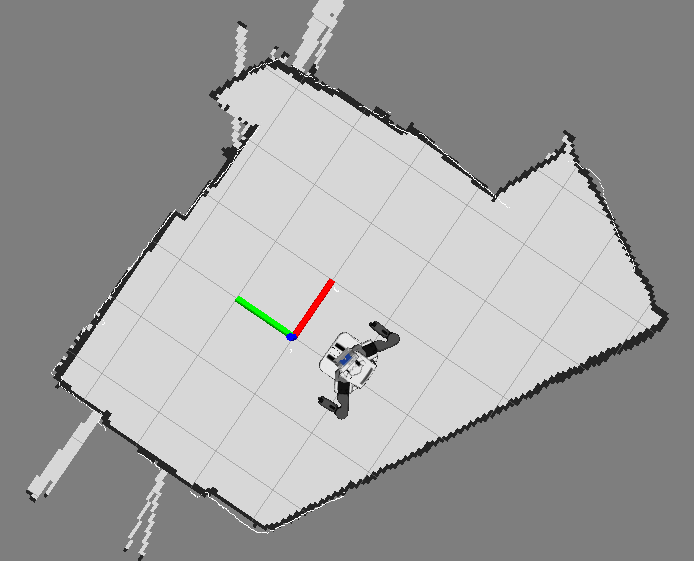
\includegraphics[width=0.59\linewidth]{./img/Map2d.png} 
  \caption {Exemple de carte pour la navigation 2-D et la localisation du robot.}
  \label{fig:map}
\end{figure}

\subsection{Objets}
% => TODO chap 23 p 543 handbook of robotics
Les lieux de travail et de vie sont également composés d'objets divers. Des récipients, des outils, des vêtements, des appareils électroniques... autant d'éléments qui peuvent prendre des formes et fonctionnalités variées.
Certains de ces objets peuvent également avoir des états. Par exemple, une bouteille peut être vide ou pleine, un vêtement peut être propre ou sale, un appareil électronique peut être éteint ou allumé.
Ces objets sont pour la plupart manipulables au cours d'une interaction. Il est donc important que le robot puisse, afin d'agir correctement sur son environnement, reconnaître ces objets et dans la mesure du possible, connaître et suivre l'évolution de leur état.

La vision permet d'obtenir des informations riches concernant les objets, en répondant aux questions "où?" et "quoi?". L'article \cite{Besl1985} propose une définition du problème de reconnaissance d'objets 3-D. Pour effectuer cette reconnaissance d'objets, diverses méthodes existent. Ces méthodes sont basées sur des solutions capteurs comme la stéréo vision \cite{murphy2005}
ou en utilisant un capteur RGBD tel la Kinect \cite{tang2012,han2013enhanced}.
%TODO? ajouter illustration reconnaissance d'objets + image Kinect
Ainsi, le robot est capable de détecter, reconnaître et positionner, moyennant une projection dans le repère global, les objets perçus par rapport au reste de l'environnement.


\subsection{Robots}
Pour comprendre la situation, le robot doit également pouvoir comprendre la situation des agents, à commencer par lui-même. 
Pour connaître sa situation, dans le cas où l'environnement est connu, le robot doit pouvoir se localiser dans l'environnement. Ceci est essentiel pour lui permettre de naviguer ou de se situer par rapport aux autres éléments.
La problématique de construire une carte de l'environnement et de localiser un robot mobile en même temps est un problème ayant été largement étudié en robotique. Ce problème est appelé SLAM (Simultaneous Localization And Mapping). Différentes méthodes existent et font l'objet de chapitre entiers dans des ouvrages tels que \cite{siciliano2008springer,thrun2005probabilistic}.
%En utilisant les éléments statiques et à l'aide de techniques de localisation,
%le robot peut également estimer sa position globale par rapport aux autres éléments de l'environnement.


Le robot est généralement composé de plusieurs membres, lui permettant de manipuler des objets, de changer son champ de vision ou de se déplacer. Il lui est donc nécessaire de connaître la configuration de ses propres membres. Cette faculté est appelée proprioception. Sur les robots, des capteurs de position permettent de transmettre la configuration des articulations, et ainsi de connaître la posture globale du robot. Le package ROS "tf"\footnote{http://wiki.ros.org/tf} peut par exemple être utilisé pour accéder aux coordonnées des articulations d'un robot, comme illustré par la figure\ref{fig:frames} où les repères des articulations d'un Pr2 sont affichées.

\begin{figure}[ht!]
 \centering
  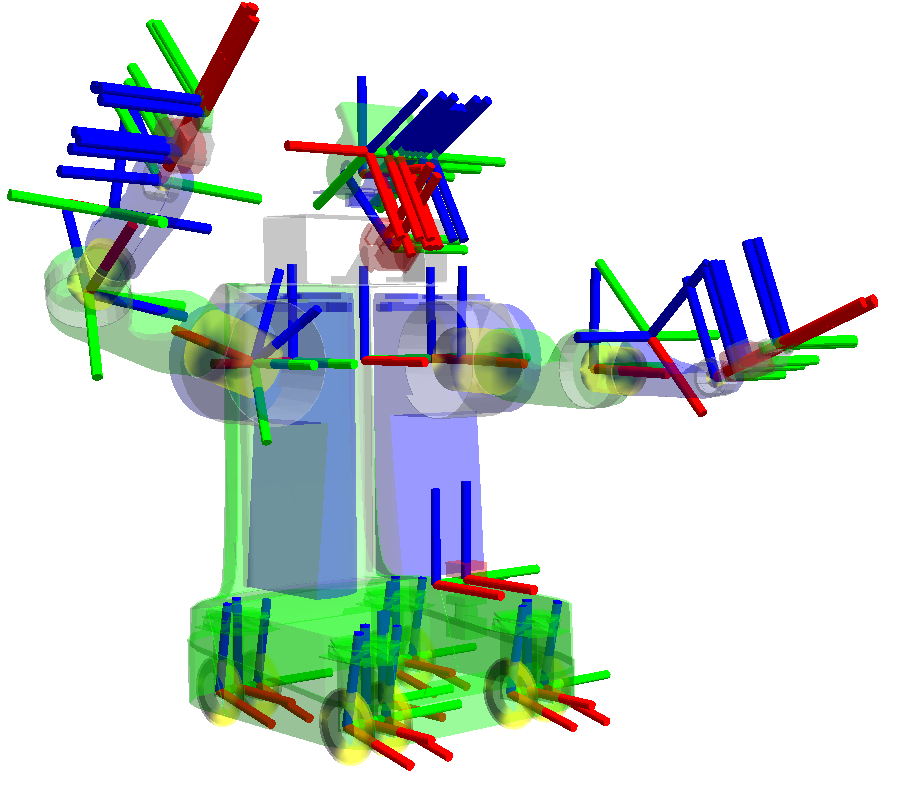
\includegraphics[width=0.59\linewidth]{./img/frames2.png} 
  \caption {Représentation des différents repères articulaires du robot Pr2 provenant de la documentation du package ROS tf.}
  \label{fig:frames}
\end{figure}

Dans le cas où l'interaction comporte plusieurs robots, différentes solutions sont possible pour connaître la configuration et la position des autres entités robotiques.
L'une des méthodes consiste à utiliser la perception. Cette méthode étant coûteuse en calcul et pas toujours fiable, l'échange direct de données est généralement privilégié. En effet, si chaque robot connaît sa position et sa configuration par rapport à un repère commun, il leur est possible de communiquer ces informations à travers le réseau et ainsi permettre à chaque robot de pouvoir accéder directement aux données des autres. Grâce à cela, il est possible à chaque système robotique de connaître la position et la configuration de chaque robot par rapport à l'environnement global.


\subsection{Humains}

Lorsqu'un ou plusieurs humains sont présents dans l'environnement, il est essentiel pour le robot de pouvoir au moins les détecter, voire de les reconnaître.
Tout comme le robot, l'homme possède plusieurs membres! Il est donc important de connaître la position de chaque homme mais aussi sa posture, et donc de percevoir la position de ses membres. Un capteur largement utilisé pour détecter les humains est la Kinect. Elle permet de connaître directement la position des différents membres de chaque humain. La figure \ref{fig:skeleton} présente la perception tridimensionnelle de la Kinect et le suivi des membres de chaque humain ainsi que l'estimation de son squelette (de la position de ses membres) calculée à partir de cette perception.

%image Kinect
\begin{figure}[ht!]
 \centering
  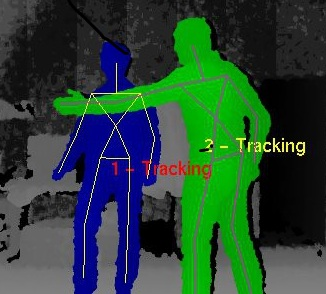
\includegraphics[width=0.59\linewidth]{./img/skeleton3.jpg} 
  \caption {Image provenant de la Kinect et illustrant le suivi des humains et de leurs membres réalisé par la librairie OpenNi.}
  \label{fig:skeleton}
\end{figure}


De même, les équipements de capture de mouvements, tel que ceux utilisés dans le cinéma d'animation, peuvent permettre d'obtenir la position et la configuration des membres des humains. Cependant cette dernière solution nécessite aux humains de s'équiper de combinaison ayant des repères visuels pour les caméras de la capture de mouvements (voir figure \ref{fig:mocap}).

%image mocap
\begin{figure}[ht!]
 \centering
  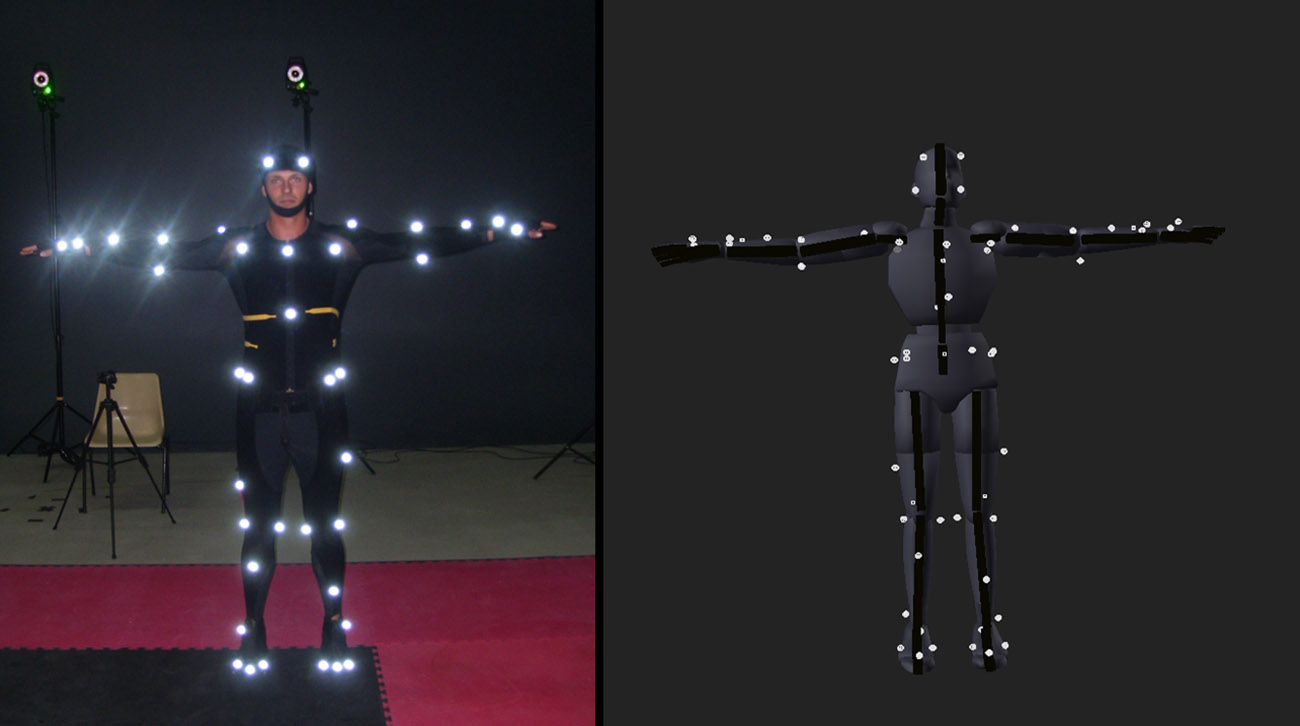
\includegraphics[width=0.69\linewidth]{./img/motionCap.jpg} 
  \caption {Exemple d'équipement de motion capture pour le suivi de l'homme et de sa posture. À gauche un homme équipé et à droite son modèle tridimensionnel.}
  \label{fig:mocap}
\end{figure}


% changer: état du monde géométrique et modélisation tridimensionnelle 
  % => aglomération des données capteurs
  % => definition de données standardisées
% Représentation des connaissances sur l'environnement: facts = diverses formes de vérité:
% état, attribut, relation spatiale...
% Calcul des connaissances
% Regroupement et Gestion temporelle des connaissances

\section{Représentation du monde et regroupement des données}
\label{sec:ws}
La seconde partie de ce premier niveau d'estimation de la situation consiste à établir une "représentation" géométrique du monde qui entoure le robot. Une fois que le système robotique peut accéder aux données de perception issues des capteurs lui permettant d'obtenir la configuration des divers éléments qui composent l'environnement, il est nécessaire, pour en extraire les informations pertinentes, de regrouper, combiner et interpréter les données. Pour ce faire, il faut dans un premier temps regrouper les données de position dans un repère commun afin que le robot puisse avoir une représentation globale de la scène. En effet, selon le capteur utilisé la position des éléments peut se faire dans le repère du capteur, du robot ou directement dans un repère global. La figure
% TODO: redo figure
\ref{fig:real} illustre cette unification avec une représentation en trois dimensions des divers éléments de l'environnement tel qu'ils sont perçus par le robot.


\begin{figure}[ht!]
 \centering
  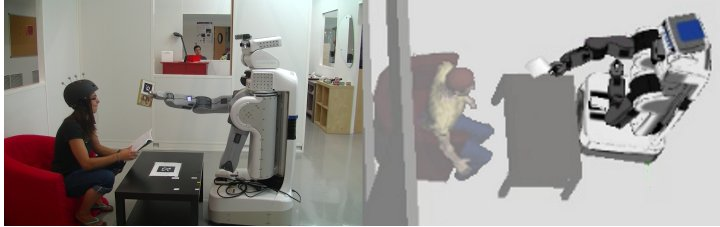
\includegraphics[width=0.99\linewidth]{./img/real2.jpg} 
  \caption {Exemple d'environnement d'interaction homme robot (à gauche), et la représentation tridimensionnelle de cette même scène tel qu'elle est perçue par le robot (à droite). La représentation utilise les données collectées des capteurs pour positionner et orienter les divers éléments dans l'environnement 3d. La représentation faite utilise le nœud de visualisation de ROS: Rviz.}
  \label{fig:real}
\end{figure}


L'unification des données capteur va permettre au système de maintenir un état du monde tridimensionnel comme dans la figure \ref{fig:real}. Pour améliorer le suivi de l'état du monde notamment au niveau des positions des divers éléments, il est parfois nécessaire d'établir un raisonnement basé sur des hypothèses, par exemple pour éviter de perdre la position d'un objet lorsqu'il n'est plus perçu. Ces raisonnements et hypothèses reposant sur des calculs géométriques et sur l'évaluation de la situation, ils seront présentés plus tard (en section \ref{sec:hypo}). 

La construction et le maintien du modèle tridimensionnel par agrégation des données provenant des divers capteurs va permettre de calculer des relations entre les différents éléments de l'environnement.
D'un point de vue architectural, le module chargé de l'unification des données capteurs est donc le module auprès du quel d'autres modules vont récupérer les données de position des éléments de l'environnement, notamment les modules d'estimation de la situation mais également d'autres tel la planification de mouvement. Il est donc important qu'il définisse les structures de données permettant de représenter l'état du monde géométrique et qu'il les rende accessibles ou les distribue aux autres modules qui en ont besoin pour raisonner sur l'environnement. Ces problématiques relèvent de l'implémentation et seront donc discutées en section \ref{sec:PDG}.


\section{Connaissances sur l'environnement et calculs de faits}
\label{sec:calculs}
\subsection{Représentation de la connaissance}
\label{sec:facts}

Pour accéder au niveau deux de connaissance de la situation décrit par Ensley, le robot doit pouvoir établir des connexions entre les divers éléments de l'environnement, connaître leur état, leur mouvements... Pour acquérir ces connaissances il est nécessaire au robot de raisonner sur la représentation du monde qu'il a construit et qu'il maintient à jour. Idéalement il doit également être capable de raisonner non seulement sur les relations spatiales et les états des éléments de l'environnement, mais également sur l'évolution de ces éléments (prise en compte de l'aspect temporel). Une fois que ces vérités relatives à l'environnement ont été calculées, le robot doit pouvoir les représenter pour les utiliser lors de la planification de tâche, de la prise de décision ou lors de dialogue avec l'homme.

Nous définissons donc un formalisme pour représenter tous ces types de vérités concernant les divers éléments de l'environnement.
Dans notre système, nous représentons l'état de connaissance du robot, aussi appelé état du monde symbolique, par une liste de \textit{faits}. Un \textit{fait} est la représentation d'une connaissance sur l'environnement traduit par une structure de données contenant divers champs. Le fait contient toujours au moins une propriété qui peut décrire l'état d'une entité, un attribut, une relation entre entité, une affordance ou tout autre vérité se rapportant à un élément de l'environnement.
Afin de décrire plus en détail cette structure de données essentielles pour notre architecture, nous énumérons ci-dessous les divers champs possibles. 

\begin{itemize}
\item \textit{Subject}\footnote{Pour éviter les confusions avec la catégorie d'éléments matériels faisant parti de l'environnement, le terme de "sujet" a été privilégié à celui "d'objet"}: l'élément de l'environnement sur lequel la propriété s'applique. Il peut s'agir d'un agent (humain ou robotique), d'un objet ou du membre d'un agent (e.g.: \textit{Red\_Mug}, \textit{Human1}, \textit{PR2\_ROBOT}, \textit{Human1\_Right\_Hand}).
\item \textit{Property}: la propriété attachée au sujet du fait (\textit{Subject}). Il peut s'agir d'une relation entre l'entité-sujet (\textit{Subject}) et l'entité-cible (\textit{Target}), d'un état ou un attribut du sujet ou plus généralement de toute vérité pouvant s'y rapporter.  Par exemple les propriétés suivantes sont utilisées dans TOASTER: \textit{isOn}, \textit{isFull}, \textit{isMoving}, \textit{isPointing}, \textit{canSee}, \textit{hasPosture}.
\item \textit{Target}: il se peut que la propriété soit une relation qui lie l'entité-sujet \textit{Subject} avec une entité-cible \textit{Target}. Par exemple, si une entité \textit{RED\_BOOK} se trouve sur une entité \textit{KITCHEN\_TABLE}, \textit{RED\_BOOK} sera alors le sujet du fait tandis que \textit{KITCHEN\_TABLE} sera l'entité-cible.
\item \textit{PropertyType}: ce paramètre définit la catégorie dans laquelle on peut classer la propriété. Il peut s'agir par exemple d'une propriété de position, d'état, de mouvement, de posture ou d'accessibilité. En utilisant ce paramètre, lorsqu'un module extérieur ajoute un fait dont la propriété est inconnue, il reste possible de savoir quel type de propriété est décrite par ce fait. Cela permet également d'appliquer certains traitements aux faits en fonction de leur type.
\item \textit{Value}: selon la propriété, il est possible qu'une valeur y soit rattachée. Par exemple, la propriété décrivant l'état d'un container \textit{isFull} ou le déplacement d'une entité \textit{isMoving} peuvent prendre la valeur \textit{TRUE} ou \textit{FALSE}. Un autre exemple, si on représente la distance entre deux membres, comme la main (ou pince) du robot et la tête de l'homme, le paramètre \textit{Value} peut contenir la valeur \textit{DANGER}, \textit{CLOSE} ou \textit{FAR}. Dans certains cas, il est également possible de donner une valeur numérique à ce paramètre.
Dans d'autres cas, pour représenter le manque de connaissances sur une propriété et le fait que ce manque est connu, la valeur du fait peut aussi être \textit{unknown}.
\item \textit{Confidence}: ce nombre entre 0 et 1 représente la fiabilité du fait. Cette valeur peut être liée à la fiabilité des capteurs ou résulter du calcul de la propriété.
\item \textit{Time}: ce paramètre permet d'enregistrer le moment auquel la propriété a été produite (perçue, calculée ou inférée).
\item \textit{FactObservability}: ce dernier paramètre représente la probabilité qu'un humain acquière la connaissance du fait s'il est capable de voir le sujet du fait. Plus de détails sur ce paramètres seront donnés dans le chapitre suivant.
\end{itemize}

Par exemple, le vecteur 
%TODO Make this as a table?
$<$ $Subject = Dan$, $Property = isMovingToward$, $Target = TABLE_4$, $PropertyType = motion$, $Confidence = 0.8$, $time = 146962814568$, $FactObservability = 0.7$ $>$ représente le fait qu'à un temps \textit{time}, l'agent \textit{Dan} se dirige vers la table du salon (\textit{TABLE\_4}). La situation dans laquelle ce fait est produit est illustrée par l'image \ref{fig:fact}.
Un autre exemple de fait correspondant à la même illustration représentant le fait que Dan est dans le salon (la zone \textit{Livingroom} en rose) prendra les champs suivants:
$<$ $Subject = Dan$, $Property = isInRoom$, $Target = Livingroom$, $PropertyType = position$, $Confidence = 0.9$, $time = 146962814568$, $FactObservability = 0.9$ $>$


\begin{figure}[ht!]
 \centering
  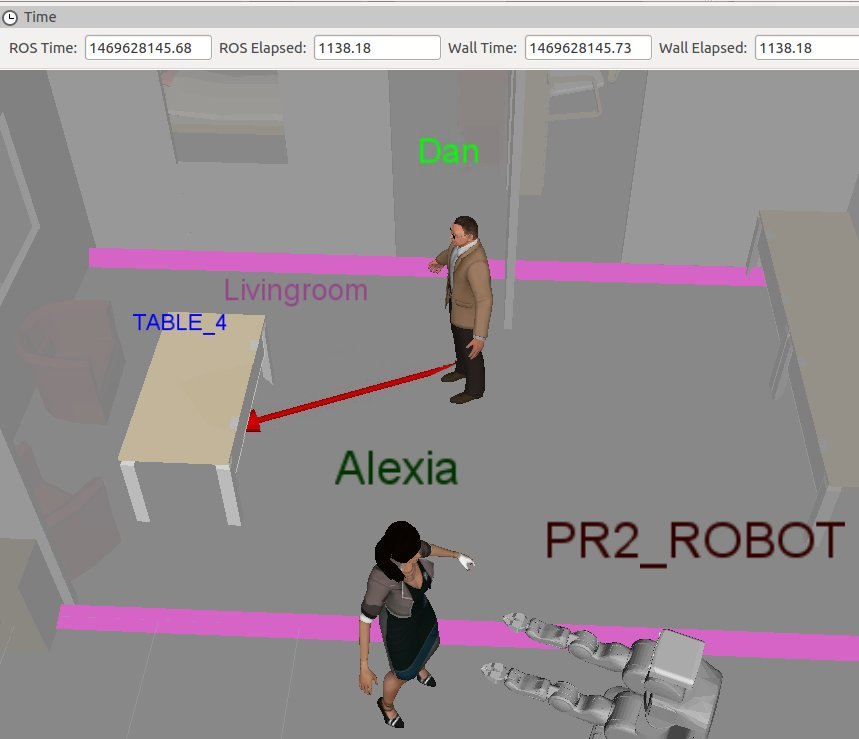
\includegraphics[width=0.99\linewidth]{./img/towardTbl.jpg} 
  \caption {Image issue de la visualisation de l'environnement et des faits dans le module de visualisation Rviz. Le fait que Dan se déplace vers la table \textit{TABLE\_4} est représenté par une flèche rouge.}
  \label{fig:fact}
\end{figure}

Les sections suivantes décrivent les raisonnements géométriques et temporels 
permettant de produire ce genre de faits.

\subsection{Calculs de faits}

Pour acquérir des connaissances sur l'environnement, il ne suffit pas de connaître la position des objets et des divers agents. En effet, il est également nécessaire d'en estimer certaines propriétés permettant de décrire leur état ou le lien qu'il peut exister entre eux. Pour ce faire, nous avons recours à une infrastructure modulaire qui en utilisant les données provenant de la perception va pouvoir calculer différentes propriétés permettant d'avoir une estimation non seulement spatiale mais également conceptuelle de l'environnement.

Nous décrivons dans les sous parties suivantes les divers outils utilisés pour produire les faits permettant de représenter cette estimation de la situation.

\subsubsection{Utilisation de zones sémantiques}
\label{sec:zones}

Pour avoir une première estimation de la situation, il est possible dans un premier temps de regarder l'emplacement des divers éléments. Pour ce faire, nous utilisons des zones ayant une signification sémantique particulière pour avoir une première catégorisation de la situation en fonction de la répartition des éléments par rapport à ces zones. Cette première estimation peut ainsi permettre de déclencher d'autres traitements afin d'optimiser les calculs nécessaires.
Par exemple il est inutile de calculer si un humain regarde le robot lorsque celui-ci est trop éloigné ou dans une autre pièce.

Nous définissons comme zone un emplacement délimité de l'environnement ayant une signification particulière. Ces zones peuvent être bidimensionnelles ou tridimensionnelles selon l'utilisation qui en est faite. Ces zones peuvent être statiques, c'est à dire liées à une position fixe dans le repère global de l'interaction, ou dynamiques, c'est à dire que la position et l'orientation de la zone est liée à un élément dynamique de l'environnement et évolue donc avec la position et l'orientation de cet élément. Pour avoir une définition générique des zones et une utilisation s'adaptant aux différents cas d'usage possible, ces zones sont paramétrables. Les paramètres permettant de définir ces zones sont:
\begin{itemize}
\item le type de la zone: ce paramètre permet de catégoriser la zone. Ainsi une zone peut-être une pièce (par exemple un salon, comme la zone rose \textit{Livingroom} à la figure \ref{fig:fact}), une zone d'interaction avec un agent (par exemple en face de l'agent en question, comme à la figure \ref{fig:interaction}), une zone de danger...
Ce paramètre permet donc de donner un contexte sémantique à la zone concernée en l'associant à une catégorie.
\item le type d'éléments concernés par cette zone: une zone peut concerner que certains éléments de l'environnement. Ce paramètre permet de définir quel type d'éléments doivent être considérés. Il peut s'agir de toutes les entités (objets, et agents), ou simplement des agents ou d'un seul type d'entité (humain, robot ou objet). Les éléments ne faisant pas partie de la catégorie choisie seront ignorés des calculs effectués en lien avec cette zone.
\item le type de calcul lié à cette zone: ce paramètre permet de définir quels calculs doivent être faits. Ces calculs seront appliqués aux éléments concernés et se trouvant à l'intérieur de la zone.
\item le "propriétaire" de cette zone: une zone peut avoir un "propriétaire". Si un propriétaire est défini, la zone est alors une zone dynamique dont la position et l'orientation évoluera avec la position et l'orientation de l'entité désignée comme propriétaire. Par exemple, il est possible de définir une zone d'interaction liée au robot par un trapèze positionné devant celui-ci. Si le robot bouge, la zone bougera avec lui pour toujours rester devant lui.
\end{itemize}

Pour reprendre l'exemple précédent et pour illustrer les différents paramètres, il est possible de définir une zone d'interaction devant le robot pour savoir si un humain se trouve dans cette zone et activer conditionnellement certains calculs, tel que l'orientation de l'humain pour savoir si celui-ci est dans une configuration permettant l'interaction.
Dans cet exemple le robot a pour identifiant \textit{PR2\_ROBOT}. La zone aura alors le vecteur de paramètres <\textit{interaction, humans, orientation, PR2\_ROBOT}>
Cette zone est illustrée par la figure \ref{fig:interaction} par une zone en jaune.
Dans l'exemple illustré, les faits (simplifiés ici) \textit{bob isInArea interaction} et \textit{bob isFacing PR2\_ROBOT} sont créés. Le robot (\textit{PR2\_ROBOT}) peut donc en déduire qu'il lui est directement possible de parler à \textit{Alexia} mais pas à \textit{Dan} (il devra par exemple commencer par l'appeler).

Les faits produis par ce module peuvent avoir la propriété \textit{isInRoom} si la zone a comme type particulier \textit{Room}, pour tous les autres types de zone le fait produit aura la propriété \textit{isInArea}.


\begin{figure}[ht!]
 \centering
  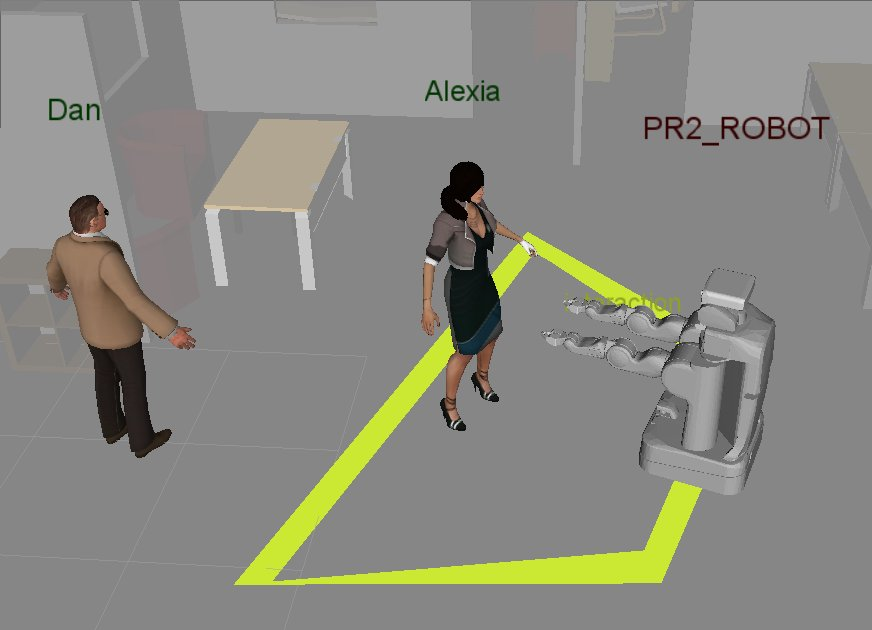
\includegraphics[width=0.69\linewidth]{./img/interactionarea.jpg} 
    \caption {Zone liée au robot Pr2 pour savoir si un humain est dans sa "zone d'interaction". Ici Alexia se trouve à l'intérieur de la zone et donc à un emplacement propice pour interagir avec le robot. Le robot va alors calculer si celle-ci lui fait face afin par exemple d'entamer un dialogue.}
  \label{fig:interaction}
\end{figure}

Ces zones peuvent être créées, mises à jour et supprimées pendant l'interaction (par exemple par le superviseur) et sont utiles pour avoir une première discrimination de la situation et des calculs conditionnels.


\subsubsection{Agencement des objets}
\label{sec:agencement}
%TODO: développer un peu plus, lister les faits...
Afin de pouvoir raisonner sur la position des objets il est nécessaire de connaître leur situation par rapport aux autres objets. Par exemple, si le but du robot est de mettre un objet sur une table, il est nécessaire qu'il puisse représenter le fait qu'un objet soit sur un autre (ici la table).

Il s'agit donc de passer d'une représentation numérique des positions à une représentation symbolique. Pour ce faire, un composant de l'infrastructure logicielle du robot calcule les relations spatiales entre les objets. Pour ce faire, ce composant utilise les modèles tridimensionnels des différents éléments stockés en mémoire pour effectuer une représentation tridimensionnelle de l'environnement. Les modèles des différents éléments sont positionnés en utilisant les données de position et d'orientation de ces éléments et leur mise à jour en temps réel pour tenir compte de l'état du monde courant (issu du processus décrit en section \ref{sec:ws}. À partir de cette représentation 3d de l'état du monde, il calcule des propriétés d'agencement spatiale pour décrire la situation des objets.

Ce composant permet de calculer si un objet O1 se trouve au dessus d'un autre objet O2 (\textit{O1 isOn O2}), dans un objet O2 (\textit{O1 isIn O2}) ou à côté d'un objet O2 (\textit{O1 isNextTo O2}) comme illustré par la figure \ref{fig:spar}. Les détails de calculs et la méthode d'implémentation proviennent de travaux précédents et sont décrits dans \cite{sisbot2011situation}.

%La méthode d'implémentation est basée sur une comparaison des bounding boxes des divers objets. Les détails de calculs 

\begin{figure}[ht!]
 \centering
  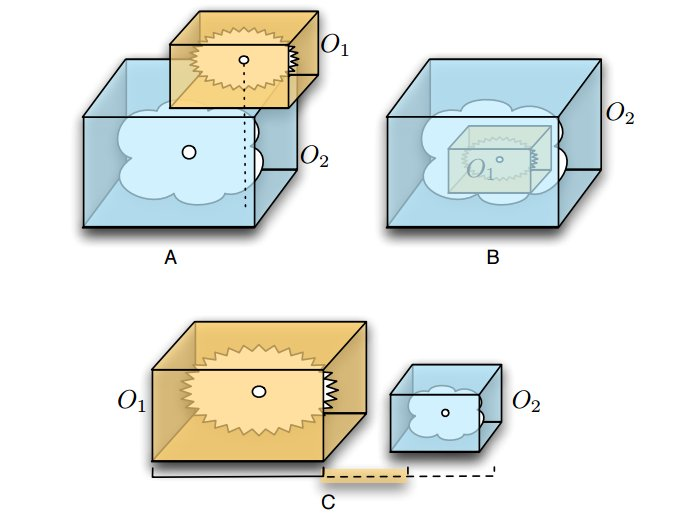
\includegraphics[width=0.5\linewidth]{./img/spar.jpg} 
  \caption {Relation spatiale entre deux objets: A) propriété \textit{isOn}, B) propriété \textit{isIn}, et C) propriété \textit{isNextTo}}
  \label{fig:spar}
\end{figure}


Grâce à ce composant il est donc possible de décrire la position de chaque objet par rapport aux autres objets de l'environnement en créant des faits avec les propriétés d'empilement (\textit{isOn}), de proximité (\textit{isNextTo}) et d'inclusion (\textit{isIn}). 

\subsubsection{Situation des agents}
\label{sec:situationAgents}

Dans un contexte d'interaction homme-robot, le robot doit accomplir des tâches en collaborant avec des humains. Il est primordial pour le système robotique d'identifier la configuration de l'humain: est-il en train de bouger? Est-ce qu'il se déplace vers un objet particulier? À quelle distance est-il de cet objet? Pour répondre à ces questions, nous utilisons un composant qui permet de surveiller chaque agent en utilisant des calculs de faits concernant les déplacements, la posture et la distance par rapport à certains points d'intérêt.

Le composant permettant de calculer ces faits enregistre en permanence les positions des entités. Afin de pouvoir stocker ces données temporairement et de les renouveler tout en évitant de surcharger la mémoire, nous avons créé une structure de données appelée buffer circulaire temporel (time stamped circular buffer). La différence avec les buffers circulaires traditionnels est que les données y sont labellisées en fonction d'un marqueur temporel et qu'il est possible d'y accéder en utilisant le temps qui leur a été attribué. Ceci permet d'accéder à la donnée de position des entités à un temps défini (moyennant de ne pas dépasser la taille du buffer).

Comme le suivi d'un agent peut s'avérer pertinent seulement dans certaines situations, le calcul des faits concernant n'importe quel agent peut être activé ou désactivé par n'importe quel autre module (en utilisant un système de requête). Ceci permet d'éviter de calculer en permanence des faits concernant tout les agents en ciblant seulement les agents qui se trouvent dans une situation nécessitant un suivi particulier.
Il est également possible d'activer le calcul de faits concernant un ou plusieurs des membres d'un agent. Lorsque le suivi d'un agent est activé, le composant calcule le déplacement de l'agent à partir des données présentes dans le buffer circulaire associé, afin de déterminer si l'agent est en train de se déplacer. En utilisant le buffer circulaire associé à l'agent et ceux associés aux autres entités, il est possible de calculer si l'agent se déplace en direction d'une entité en particulier (même si cette dernière est également en cours de déplacement) et l'évolution temporelle de la distance entre l'agent et un point d'intérêt. Ce calcul peut être aussi bien fait sur la position globale de l'agent ou sur l'un de ses membres (par exemple sur la main de l'homme).
Pour effectuer ce calcul, nous combinons deux méthodes: la première consiste à calculer la trajectoire de l'agent (respectivement de son membre) et de considérer que les entités se trouvant dans cette direction, moyennant une marge d'erreur paramétrable, sont des candidats potentiels. La seconde méthode utilise le différentiel de distance entre l'agent et les entités candidats. Si la distance diminue, l'agent se rapproche de l'entité. En combinant ces deux méthodes de calculs, on peut avoir une liste de candidats avec un coefficient de confiance pour les entités vers lesquelles l'agent se déplace. Ce calcul est évidemment simpliste car il ne prend pas en compte les éventuels obstacles qui pourraient faire qu'un agent fait un détour pour se diriger vers une entité. Cependant il permet dans de nombreux cas d'avoir une idée de l'entité vers laquelle l'agent se déplace.

En plus du mouvement, nous calculons également les distances entre les agents surveillés (respectivement les membres surveillés) et les autres entités.
De cette manière il est possible de savoir si un humain, ou l'un de ses membres, est proche d'un point d'intérêt (comme le robot ou un objet avec lequel il veut interagir).
Par exemple, ce module peut produire les faits (simplifiés ici) <\textit{HUMAN1 isMoving TRUE}> pour indiquer que l'humain \textit{HUMAN1} est en mouvement ou <\textit{HUMAN1\_RIGHT\_HAND isMovingToward BLUE\_BOOK}> pour indiquer que la main droite de l'humain se dirige en direction du livre bleu.

Le dernier type de fait concerne la posture de l'agent. En utilisant le buffer circulaire il est possible de savoir vers quoi l'humain pointait le doigt à un instant donné. Ceci peut être utile par exemple pour un module de fusion d'un système de dialogue. Ainsi, si un humain demande au robot "donne-moi ça", si la reconnaissance de parole est capable de fournir le temps pour lequel le mot "ça" a été prononcé, il est possible de demander au module quel(s) objet(s) étai(en)t pointé(s) par l'humain au moment où il a prononcé le mot "ça". Pour alléger la charge de calcul, ce fait est calculé seulement sur demande (et non en permanence comme les autres). Le module utilise la position de la main de l'agent par rapport à son épaule pour calculer la direction de pointage. Tous les éléments se trouvant dans cette direction, à un angle d'erreur prêt, sont renvoyés dans une liste d'entités avec un indice de confidence basé sur l'angle de déviation par rapport à la direction pointée, pour chaque élément de la liste.




\section{Hypothèses pour le maintien de l'état du monde}
\label{sec:hypo}
\subsection{Hypothèses de position}
%Put this in maintien du monde 3D?
%9.2 p 213 of handbook
% que faire lors de contradiction entre connaissance et perception?
% solution = faux positifs faible ou inexistant => perception privilégiée


Dans leur quotidien, les humains sont occupés par divers activités (cuisine, nettoyage, bricolage...). Ces activités impliquent très souvent l'utilisation d'objets. Comme les robots sont fait pour assister les hommes dans leurs tâches quotidiennes, il est crucial qu'ils puissent non seulement manipuler les objets, mais également suivre leur changement de position. Notre but ici n'est pas de discuter des différentes méthodes de suivi d'objet basées sur la perception mais d'expliquer comment le raisonnement sur les données de perception peut améliorer la détection et le suivi d'objet.

Localiser et suivre un objet n'est pas une tâche simple. En effet, l'objet peut être de petite taille et par conséquent être fréquemment occulté ou hors du champ visuel.
Les humains sont capables de connaître la localisation d'un objet même sans perception directe. Ils font en permanence des hypothèses sur la position des objets qu'ils ne peuvent pas voir et effectuent des raisonnement basés sur ces hypothèses. Pour travailler efficacement avec des humains, le robot doit être capable lui aussi de faire ce genre de raisonnements.

Pour ce faire, nous avons ajouté au composant qui maintient à jour l'état du monde, la possibilité d'émettre des hypothèses de position lorsqu'un objet n'est pas visible.

Comme hypothèse de base, lorsque le robot est dans l'incapacité de voir l'objet (l'objet est hors du champs de vision ou est caché), le système suppose que l'objet est à la même place et a la même orientation que la dernière fois qu'il l'a perçu. Dans la figure \ref{fig:occluded}, dans la configuration où le robot perçoit les objets à partir de caméras au niveau de sa tête, 
le livre bleu étant caché par la boîte rose, il n'est pas visible par le robot. Cela signifie que le capteur de vision n'est plus capable de fournir la donnée de position de cet objet. Cependant, en utilisant la représentation 3d et des calculs de visibilité, il est possible pour le robot de savoir que l'objet n'est pas visible à sa position courante. Le système de maintien de l'état du monde le conserve tel quel dans le modèle de l'environnement car il sait que l'objet est caché, et qu'il est donc normal qu'il ne soit pas détecté. Cette hypothèse de maintien de position est utilisée comme hypothèse par défaut. Cela signifie que s'il y a une autre hypothèse concernant la position d'un objet, nous choisirons cette dernière plutôt que celle par défaut.
Ainsi, si l'on reconnaît une action d'un agent qui consiste à prendre cet objet, l'hypothèse que l'objet est dans la main sera privilégiée.

\begin{figure}[ht!]
 \centering
  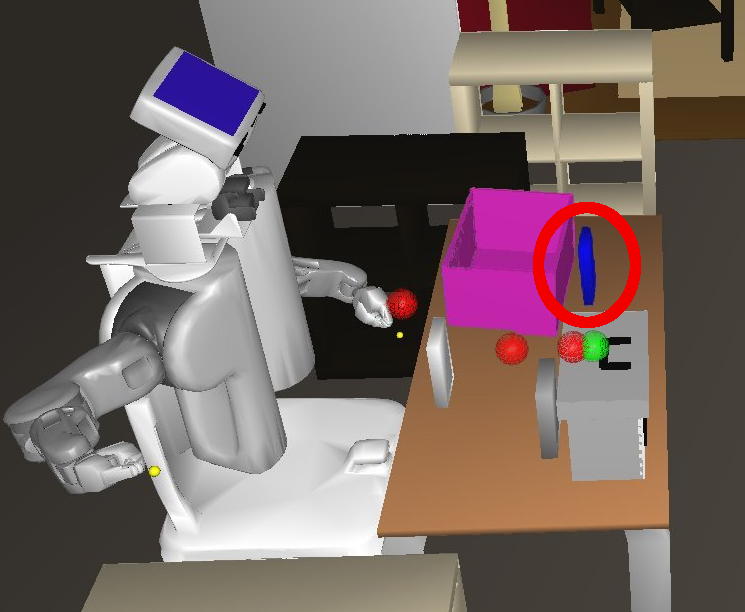
\includegraphics[width=0.69\linewidth]{./img/occluded.png} 
  \caption {Exemple d'État du monde où le système maintient les objets en position même s'ils ne sont pas directement perçus (comme le livre bleu). Ici le robot a une perception uniquement basée sur des caméras placées dans sa tête.}
  \label{fig:occluded}
\end{figure}

Les autres hypothèses de position sont créées à partir des actions du robot et de l'homme. Si le robot attrape un objet, l'objet sera probablement caché par sa propre main, mais nous savons où l'objet se trouve (dans la main du robot). Par ailleurs, sur certaines plateformes robotiques, ce type d'hypothèse peut être confirmer en utilisant des capteurs d'effort au niveau de la main du robot ou en mesurant l'ouverture après fermeture pour confirmer la présence d'un objet.

Nous avons le même type d'hypothèse pour l'humain, en utilisant les observations sur la situation de l'humain (proximité avec un objet, posture, mouvement) présentées à la section \ref{sec:situationAgents}, il est possible de suivre les actions de l'homme, et ainsi de savoir quand un humain prend un objet ou le dépose.

En dernier lieu, nous avons également une hypothèse permettant de connaître la position des objets lorsque ceux-ci sont contenus dans d'autres objets.
Si un agent laisse tomber un objet dans un autre, même si il n'est pas possible de voir l'objet lâché, il est possible d'approximer sa position (par exemple en le mettant au centre du contenant).

\begin{figure}[ht!]
 \centering
  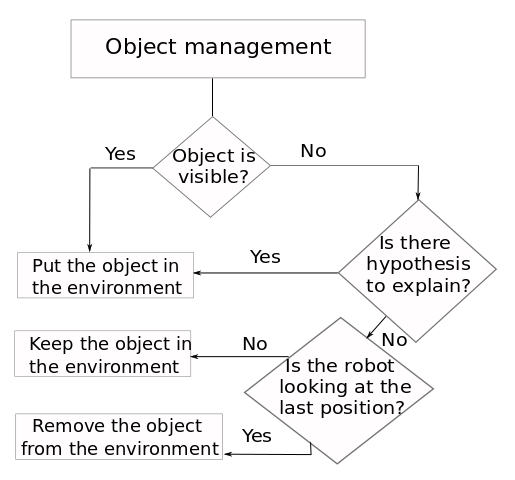
\includegraphics[width=0.70\linewidth]{./img/hypothesis.png} 
  \caption {Schéma de raisonnement pour gérer la position d'un objet. Les hypothèses sur la position des objets peuvent provenir d'une occlusion, d'un objet dans un conteneur ou dans la main d'un agent.}
  \label{obj_manag_fg}
\end{figure}

Pour résumer, le robot utilise en premier lieu la perception, puis s'il n'est pas possible de percevoir l'objet il utilise des hypothèses de position.
Si aucun des deux n'est disponible, il utilise la dernière position de l'objet, comme indiqué par la figure \ref{obj_manag_fg}.
Les hypothèses de position doivent être gérées en temps réel pour maintenir un modèle du monde cohérent.
Dans le cas où un objet a une hypothèse de position et est perçu en même temps, la position perçue est comparée avec celle donnée par l'hypothèse de position. Si la  position indiquée est incompatible (distance trop importante) l'hypothèse est alors supprimée car elle est considérée comme impossible.
Si un objet devrait pouvoir être perçu et ne l'est pas, alors l'hypothèse par défaut est annulée et la position de l'objet prend alors la valeur "unknown" pour indiquer que le robot ne sait pas où se trouve l'objet en question.

Ces hypothèses concernant la position des objets liés à un raisonnement top-down (symbolique vers sub-symbolique) permettent au robot d'avoir un suivi plus efficace des objets, spécialement quand ils sont occultés ou non perçus et ainsi avoir une représentation de l'état du monde plus fiable en palliant à certaines limitations de la perception.


\subsection{Généralisation}


%TODO: généralisation du maintient du monde par la gestion des hypothèses (rempli / vide, chaud/froid...)
% Différent car ne modifi pas l'état du monde sub symbolique
%http://link.springer.com/article/10.1007%2Fs13218-015-0400-1

Pour aller plus loin, nous travaillons actuellement à généraliser ces hypothèses. En effet, il est important de pouvoir suivre la position des objets, et donc d'établir des hypothèses pour pallier le manque de visibilité et avoir un suivi efficace de la position des objets, mais il est également important de connaître l'état des divers propriétés liées aux objets. Contrairement aux hypothèses de position, ces hypothèses n'influencent pas la représentation tridimensionnelle de la scène mais uniquement les données symboliques.

Dans l'environnement, nous considérons que seul les agents peuvent agir pour modifier l'état du monde. Ainsi dans cette première approche, nous ne prenons pas en compte l'évolution temporelle de certaines propriétés (comme par exemple le fait qu'une boisson chaude refroidisse).
Le maintien des hypothèses concernant les faits symboliques décrivant l'état du monde est donc effectué à partir du suivi des agents et de l'estimation de leurs actions. Nous utilisons pour cela un module de reconnaissance d'actions appelé AIR (Action and Intention Recognizer), dont le fonctionnement est présenté au chapitre \ref{chapter4}.
Ce module transmet au module de gestion d'hypothèses (Hypotheses Manager) les actions détectées par le système.
De nombreux travaux traitent de la question de la mise à jour du monde à partir de la reconnaissance d'actions \cite{ginsberg1988reasoning,ginsberg1988reasoning2,rao1989minimal,jackson1990semantic,brewka1993things}.
Ainsi, dans l'infrastructure de représentation de connaissances KnowRob, des \textit{règles de projection} sont utilisées pour connaître l'état du monde après qu'une action se soit réalisée \cite{tenorth2015representations}. Les actions peuvent changer la position des objets mais également le détruire ou créer un nouvel objet en combinant deux autres (par exemple en mélangeant deux ingrédients). Ici, nous traitons uniquement des actions pouvant modifier la position (comme présenté précédemment) ou l'état d'un objet, comme par exemple le fait de remplir ou vider un container, de nettoyer un objet ou encore de l'allumer ou l'éteindre. L'idée est d'associer à chaque action un effet (se traduisant par la modifications de certains faits symboliques) dont l'action est la cause. Cet effet est aussi appelé post-condition. Basé sur les posts-conditions de l'action reconnue, le module de gestion d'hypothèses est capable de mettre à jour certains faits liés à l'état symbolique du monde pour prendre en compte l'effet de l'action reconnue.

Par exemple, si le module AIR détecte qu'un humain a versé le contenu \textit{C} d'un récipient \textit{B} (comme une bouteille) dans un autre récipient \textit{V} (comme un verre), le rôle du module de gestion des hypothèses sera d'envoyer une requête à la base de données pour mettre à jour l'état des propriétés liées à \textit{V} et \textit{B}. Ainsi, la propriété \textit{isEmpty} sera mise à faux pour \textit{V} et la propriété \textit{hasLiquid} sera ajoutée avec \textit{C} comme valeur (\textit{C} peut être par exemple de l'eau). Le module de gestion d'hypothèses sera également chargé de décrémenter la quantité de \textit{C} contenue dans \textit{B}.
Pour résumer, ce module de gestion d'hypothèses permet d'appliquer les effets (ou postconditions) liés à une action lorsque celle-ci est détectée. Il sera également en charge d'assurer la cohérence globale de l'état du monde.


Le schéma \ref{fig:hypo} présente l'architecture permettant cette gestion d'hypothèses. Le module de gestion d'hypothèses peut communiquer avec le module d'agrégation de données et de maintien du monde (Perceived Data Gathering) pour modifier la position d'un objet, ou avec la base de données temporelle (présentée à la section suivante) pour modifier certains faits, et donc l'état du monde symbolique.

\begin{figure}[ht!]
 \centering
  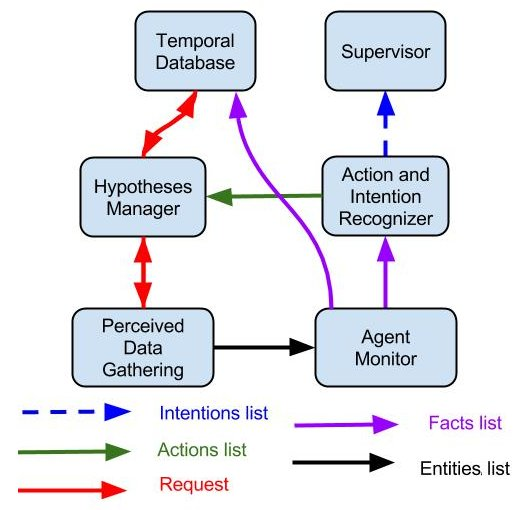
\includegraphics[width=0.7\linewidth]{./img/hypotheses_manager.jpg} 
  \caption {Schéma de l'architecture prévisionnelle pour le module de gestion des hypothèses.}
  \label{fig:hypo}
\end{figure}


%TODO: Temporal database here?
\section{Base de données temporelle}
\label{sec:db}
%%%%%%%%%%%%%%%%%%%%%%%%%%%%%%%%%%%%%%%%%%%%%%%%%%%%%%%%%%%%%%%%%%%

%http://journal.frontiersin.org/article/10.3389/frobt.2015.00019/full
%Open ease

Nous avons présenté précédemment comment divers composants contribuent à maintenir un état du monde géométrique (sub-symbolique). Nous avons également présenté comment d'autres composants, à partir de l'état du monde géométrique et de raisonnements et calculs sur celui-ci, produisent une liste de faits permettant une représentation symbolique de l'état du monde et une estimation de la situation.

Afin de regrouper ces données symboliques et permettre un accès standardisé et efficace, nous avons ajouté une base de données SQL à notre système.

\subsection{Gestion des données}
\label{sec:dbd}
La base de données peut gérer deux types de données: les données statiques et dynamiques. En effet, il est possible de connaître à priori certaines informations sur l'environnement tel que la couleur, le nom de certains objets ou leur type ou leur propriétaire. 
Nous avons donc dans notre base de données une première table permettant d'avoir des informations sur les diverses entités de l'environnement. Cette table peut être complétée en ligne si le système reçoit des informations complémentaires durant l'interaction (si le robot découvre de nouvelles propriétés statiques ou de nouveaux objets, que se soit par la perception ou le dialogue).

Concernant les données symboliques et notamment les \textit{faits} produits par les divers composants d'évaluation de la situation, la base de données récupère en permanence la liste de faits produite et publiée par chacun des modules. Cela permet de vérifier les changements apparus dans l'environnement pour mettre à jour la table de représentation symbolique de l'état du monde tel qu'il est perçu par le robot (\textit{ROBOT\_WS\_TBL} pour Robot World State Table).
Cette table est composée de faits qui sont considérés comme vrais et mis à jour en temps réel. Ces faits proviennent des divers modules d'évaluation de la situation et ont comme valeur temporelle la date où le fait a été détecté.

%blabla etat du monde + données statiques

\subsection{Gestion de la temporalité}
\label{sec:dbt}
%TODO: open ease http://ieeexplore.ieee.org/stamp/stamp.jsp?arnumber=7139458
L'une des valeurs ajoutées de cette base de données est l'aspect temporel.
Ceci permet de doter le système d'une mémoire des faits passés.
Dans \cite{vernon2014artificial}, Vernon décrit la mémoire des systèmes cognitifs comme un moyen de "facilité la persistance des connaissances et forme un réservoir d'expérience".
Ainsi, certains systèmes de gestion de connaissances intègrent des mécanisme de mémoire et de raisonnement sur la mémoire, tel KnowRob \cite{tenorth2015representations} ou encore Open-Ease \cite{beetz2015open}.
Open-Ease est une base de connaissance en ligne fournissant des données sur les activités des humains et des robots. Open-Ease fournit également un langage pour effectuer des requêtes sur la base de données ainsi qu'un système d'inférences. Cela permet au robot de répondre aux questions sur leur propres actions en fournissant les raisons et en décrivant les différentes étapes.

Dans notre implémentation, la mémoire est principalement réalisée en terme de sauvegarde d'état précédent des propriétés et des événements s'étant produits dans l'environnement.
En effet, lors d'une interaction homme-robot, de nombreux événements peuvent se succéder et pour pouvoir comprendre et interpréter les actions et les élocutions de l'homme, il est important de considérer l'historique de l'interaction.

Nous avons donc ajouté une gestion de l'aspect temporel.
Pour ce faire, lorsqu'un fait est considéré comme vrai à partir d'un temps t1 et donc présent dans la table de représentation symbolique de l'état du monde perçu par le robot, le temps t1 lui est attribué jusqu'à ce que ce fait soit considéré comme faux à un temps t2.

Lorsque le fait est considéré comme faux en t2, ou lorsqu'il change de valeur, il est retiré de la table \textit{ROBOT\_WS\_TBL} pour être mis dans une table mémoire \textit{ROBOT\_MEM\_TBL}. Cette table contient également une liste de faits. À la différence de la table \textit{ROBOT\_WS\_TBL}, les faits de cette table peuvent être en double (deux faits identiques peuvent être présent dans la table si ils ont des temps différents) et représentent des faits passés. Pour ce qui est du temps associé, chaque fait a deux dates: la date t1 à laquelle le fait a commencé a être vrai (ou plutôt détecté comme étant vrai) et la date t2 à laquelle le fait a cessé d'être vrai (détecté comme étant faux).
Pour avoir un accès direct aux transitions, nous avons également ajouté une table d'événements \textit{EVENT\_TBL}. Lorsqu'une transition de fait est détectée (un fait n'est plus vrai ou change de valeur), en plus de le retirer de la table de faits courant et de l'ajouter à la table mémoire, nous ajoutons la transition avec la date de t2. 

Pour illustrer, nous prenons l'exemple où un homme \textit{H} prend un objet \textit{O} sur une table \textit{T} à un moment t2. Trois opérations seront faites dans la base de données:

\begin{itemize}
\item Le fait \textit{O isOn T} sera déplacé de la table \textit{ROBOT\_WS\_TBL} vers la table \textit{ROBOT\_MEM\_TBL}, avec t2 comme temps de fin.
\item Le fait  \textit{H hasInHand O} sera ajouté à la table \textit{ROBOT\_WS\_TBL} avec un temps t2.
\item L'événement \textit{H picks O} sera ajouté à la table \textit{EVENT\_TBL}.
\end{itemize}

Cette gestion du temps, des événements et de la mémoire permet de pouvoir réaliser des raisonnements temporels complexes sur les données symboliques et les liens temporels entre les différents faits. L'une des améliorations à venir est de permettre "d'oublier" les événements en fonction de leur date et de leur ancienneté pour éviter de saturer la mémoire dans le cas d'une utilisation longue durée.



% %TODO: improve clearness
% Another capacity of the database component is the event based time management. This provides memory to the system.
% When facts are received, the time of detection is present in one of their variables (as mentioned in \ref{sec:facts}). When the database manager detects a shift in a property, it updates the belief tables as explained in previous section, but it also records the event. To do so, we add a table filled with each event that occurs, recording the time when the property changes. As an example, if a Mug was on a table and the robot detects that the Mug is now in Bob's hand, it will remove the fact $<$\textit{Mug isOn $Kithen\_Table$}$>$ from the belief tables of agents able to perceive the change, and add the event $<$\textit{Bob pickUp Mug}$>$ in the event table.
% In addition to the event table, we add a memory table for each agent. This memory table stores facts that the agent has believed to be true. We use as starting time the time when the agent noticed a property, and as ending time the moment when the agent detects a change in it.
% One of the application can be to 
% %find correct terminology: reference finding? grounding? desambiguate?
% %Miki: This is quite nice actually. What about making real experiments on that? XD
% %Greg: Yep, we should! I put it in the conclusion
% %But we also have to work on robustifying the thing...
% understand when a human asks "Where is the mug that was on the table" by detecting in his memory table which mug she/he is talking about and looking in the current fact table where it currently is. In addition, the robot could even tell the related event that created the change: "It is now in the sink, Bob picked it up 5 minutes ago".



%%%%%%%%%%%%%%%%%%%%%%%%%%%%%%%%%%%%%%%%%%%%%%%%%%%%%%%%%%%%
\section{Implémentation}
\label{sec:impl}

Les composants décrits précédemment ont été implémentés dans une infrastructure logicielle open-source appelée TOASTER\footnote{TOASTER est disponible sur github à l'adresse https://github.com/Greg8978/toaster} (Tracking Of Agents and Spatio-TEmporal Reasonning).

L'un des avantages de TOASTER repose sur sa généricité et son adaptabilité grâce à une conception modulaire qui permet également d'étendre facilement l'infrastructure. En effet, comme présenté en section \ref{sec:collecte}, les données d'environnement peuvent parvenir de divers capteurs.

\subsection{Collecte de données et généricité}
\label{sec:PDG}
Pour que l'infrastructure logicielle soit utilisable avec n'importe quelle configuration de capteurs, un premier module permet de collecter toutes les données et de les mettre au format TOASTER. Tous les autres modules utiliseront ensuite l'état du monde au format exporté par ce module. Ce module chargé de collecter les données des divers capteurs est appelé \textit{PDG} pour Perceived Data Gathering.
Il permet à l'heure actuelle de gérer quatre types d'entrées pour l'homme, deux pour les objets, deux modèles de robot. Il gère également, à l'heure actuelle, la lecture de deux types de messages: les topics ROS\footnote{http://www.ros.org/} et les posters pocolibs \footnote{https://www.openrobots.org/wiki/pocolibs}.

Un autre avantage de ce module est également sa simplicité d'extension. Ainsi, grâce au système d'héritage du C++ il est possible d'ajouter une entrée capteur pour détecter des objets, pour suivre l'homme ou un modèle de robot en seulement 50 à 200 lignes de code C++ (estimation basée sur les entrées déjà existantes).
Au démarrage du module ou à tout moment de l'interaction, il est possible de (re)configurer se module pour modifier les entrées à prendre en compte.

Durant la phase de développement de nouvelles fonctionnalités il est coûteux d'un point de vue matériel tout comme d'un point de vue temporel de faire des tests dans le monde réel. Pour permettre de tester rapidement et sans monopoliser de plateforme robotique, le module \textit{PDG} peut prendre en entrée des données de simulateur robotique tel que Gazebo\footnote{http://wiki.ros.org/gazebo} pour la configuration du robot, MORSE\cite{echeverria11} pour la configuration de l'homme, du robot et la vision des objets. En plus de ces simulateurs, un module intégré à TOASTER pour créer et tester des environnements d'interaction homme robot appelé \textit{toaster\_simu} a été créé. \textit{PDG} permet également d'avoir une configuration hybride.
Par exemple, il est possible d'utiliser les capteurs d'un robot réel ainsi que la détection d'objets dans le monde réel et de simuler le déplacement d'un humain (avec l'interface clavier).
Le module \textit{PDG} permet donc une grande flexibilité dans la configuration des données d'entrées. En exportant l'état du monde dans un format unique et invariable, \textit{PDG} permet aux autres modules TOASTER de s'abstraire de cette diversité et de conserver les mêmes formes de raisonnement, indépendamment de la configuration des capteurs et des données d'entrées de TOASTER.

\subsection{Outils de développement}
Pour aider au développement de nouvelles fonctionnalités et à la configuration de scénarios, un module de visualisation a été ajouté à l'infrastructure TOASTER. Ce module utilise le système de visualisation intégré à ROS, Rviz\footnote{http://wiki.ros.org/rviz} pour afficher les différents éléments en trois dimensions, ce qui permet de comprendre la situation en affichant l'état du monde. Chaque entité est associée à un modèle 3D qui est positionné dans un environnement virtuel à la position et à l'orientation données par le module PDG. Le module affiche également les noms de chaque entité au dessus de leur modèle 3D. 
Le module permet également d'afficher les différentes zones présentes dans le module de gestion de zone (\textit{area\_manager}) avec leurs noms, comme présentée sur la figure \ref{fig:interaction}.
Concernant les faits exportés par le module de suivi d'agents (\textit{agent\_monitoring}), afin d'éviter la surcharge de l'interface, le fait \textit{isMoving} rend l'affichage du nom de l'agent plus intense selon si le système considère qu'il bouge. La donnée numérique de sa vitesse associée à ce fait permet également de faire varier cette intensité. Pour le fait \textit{isMovingToward}, une flèche reliant l'agent à l'entité vers laquelle il se déplace est tracée. L'intensité de la couleur de cette flèche varie également en fonction de l'indice de confiance du fait associé. Ce retour visuel est illustré par un exemple à la figure \ref{fig:moving}

\begin{figure}[ht!]
 \centering
  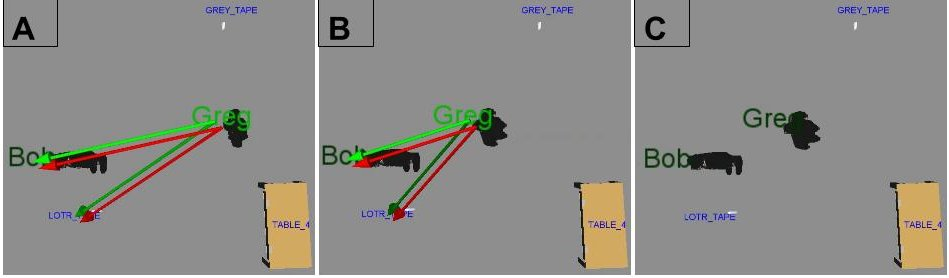
\includegraphics[width=1.0\linewidth]{./img/movingToward.jpg} 
  \caption {Affichage dans Rviz des faits liés au module \textit{agent\_monitoring}. La flèche rouge indique ce fait calculé en terme de différentiel de distance alors que la flèche verte indique ce même fait en terme de direction de trajectoire. Sur l'image A et B \textit{Greg} se déplace vers \textit{Bob} ainsi que vers un objet (\textit{LOTR\_TAPE}). Sur l'image A et de façon plus prononcée sur l'image B, les flèches allant vers \textit{LOTR\_TAPE} sont plus sombres, indiquant que la confidence pour ce candidat est moins grande que pour \textit{Bob}. En C Greg s'est arrêté. Les flèches de directions sémantiques ont disparues et le nom de Greg s'est assombri (pour devenir comme celui de Bob qui est immobile).}
  \label{fig:moving}
\end{figure}

Cette visualisation permet de comprendre l'état du monde tel qu'il est perçu par le robot et permet donc de faciliter les explications liées aux agissements du robot, mais aussi de faciliter la configuration d'une nouvelle expérimentation et la recherche d'erreurs lors de l'implémentation de nouvelles fonctionnalités. 

%It uses the position of the entities published by the data gathering component and the areas published by the area manager component as shown in Fig.~\ref{fig:simu} and Fig.~\ref{fig:spencer}. In a future work, we would like to improve this visualization by adding the rendering of other facts, such as the one generated by the agent monitoring component.

Un autre composant déjà évoqué dans la partie \ref{sec:PDG}, permettant de rapidement paramétrer et tester des expérimentations est le module de test \textit{toaster\_simu}. Grâce à ce module, il est possible par une simple requête d'ajouter et positionner des entités dans l'environnement. Il est également possible de contrôler ces entités par une interface clavier. Le module exportera alors en temps réel les données liées à l'état du monde créé par l'utilisateur et ces données seront lues par le module PDG. Il est donc possible, à partir d'un simple script envoyant quelques requêtes, de configurer un environnement d'interaction avec des robots, des humains et des objets. Des scripts Python pour configurer un environnement de simulations sont disponibles à titre d'exemple\footnote{https://github.com/Greg8978/toaster-scripts}.


\subsection{Architecture globale}
Les autres modules compris dans l'infrastructure logicielle TOASTER ont une implémentation qui suit les descriptions données précédemment.
Ainsi, le module \textit{area\_manager} permet d'ajouter et de supprimer des zones dans l'environnement à l'aide de requêtes. Le modèle et les raisonnements développés dans ce module suivent la description faite en \ref{sec:zones}. Pour le calcul de l'agencement des différents éléments, un module nommé \textit{SPAR} (pour SPAtial Reasonning) est utilisé. Enfin, pour le suivi des agents décrit en \ref{sec:situationAgents}, le module \textit{agent\_monitoring} a été développé.
Concernant la base de données temporelle, nous avons conçu celle-ci en utilisant la bibliothèque SQLite\footnote{https://www.sqlite.org/}. Ce choix a été fait car cette base de données est très répandue, respecte les conventions SQL et permet une gestion in-memory des données qui augmente les performances en terme de vitesse d'accès à la donnée.

Chacun de ces modules peut être démarré et arrêté à n'importe quel moment de l'interaction. Il peut également recevoir des requêtes ou des messages provenant d'autres composants mais ne dépend pas directement des autres. Par exemple, il est possible d'utiliser le module de raisonnement sur les zones (\textit{area\_manager}) sans \textit{PDG}. Cependant il est nécessaire, si l'on veut que les calculs sur la présence d'entités dans les zones soit effectif, que le module \textit{area\_manager} reçoive les données correspondantes.
De même, la base de données temporelle a été conçue pour pouvoir lire des listes de faits en entrée mais il est possible de paramétrer celle-ci afin de définir quelles listes de faits doivent être lues.
Ceci permet de facilement remplacer un module de l'architecture sans impacter les autres modules, dans la mesure où ce nouveau module respecte les conventions de formats de données d'entrée et sortie.

Pour aider à la compréhension, nous proposons le schéma d'architecture \ref{fig:toasterArch} qui présente comment les données des différents composants peuvent s'interfacer.


\begin{figure}[ht!]
 \centering
  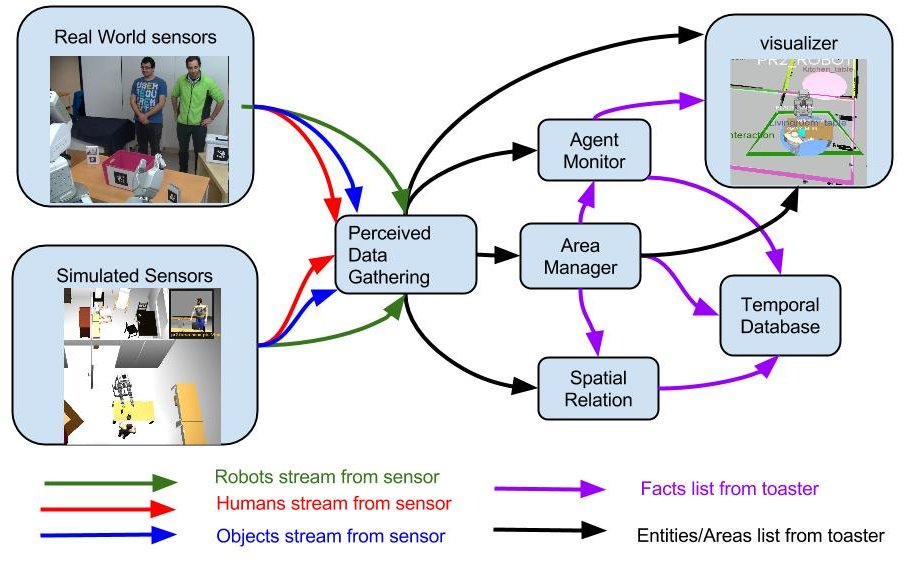
\includegraphics[width=0.99\linewidth]{./img/toasterArch.jpg} 
  \caption {Architecture de l'infrastructure logicielle TOASTER avec les différents flux d'échanges de données}
  \label{fig:toasterArch}
\end{figure}

\section{Résultats expérimentaux}
Pour illustrer l'utilisation possible de TOASTER, nous présentons ici deux expérimentations utilisant l'infrastructure logicielle.

\subsection{Le robot guide}

L'une des premières applications de TOASTER a été de l'utiliser comme composant d'estimation de la situation pour un robot guide adaptatif, proactif et prenant en compte les humains \cite{fioreicsr2015}.

Pour cette application, le robot doit guider un groupe d'utilisateurs à travers une zone de transit (potentiellement bondé), pour les amener à l'endroit choisi.
L'un des défis de ces travaux était de guider les personnes de façon socialement acceptable et en prenant en compte le confort des usagers.
Le robot adapte sa vitesse au groupe, afin de tous les amener à leur destination avec une allure qui satisfasse la plupart des usagers et évite que certains utilisateurs n'abandonnent.

Pour atteindre ces objectifs, nous avons utilisé: (1) le module PDG pour regrouper les données capteurs afin de créer et maintenir le modèle de l'état du monde; (2) les faits produits par le module de gestion des zones (area\_manager); (3) les faits produits par le module de suivi des agents (agent\_monitoring), pour comprendre la situation du groupe. 

Concernant le module de gestion des zones, deux types de zones ont été crées: les zones de guidage et les zones d'activité. Les premières sont liées au robot et évoluent donc avec sa position et son orientation. Elles sont utilisées pour évaluer la configuration des utilisateurs par rapport au robot guide, ce qui lui permet d'adapter sa vitesse en fonction de la configuration du groupe.
L'idée est de créer trois zones de guidage autour du robot pour savoir si la configuration des utilisateurs indique qu'ils souhaitent que le robot aille plus vite ou si l'un d'entre eux a du mal à suivre.
Les trois zones sont appelées \textit{slow}, \textit{following} et \textit{pushing} et sont configurées comme indiqué dans la figure \ref{fig:spencer}.
L'idée est que, (1) si l'un des membres du groupe est dans la zone \textit{slow} (loin du robot) le robot \textit{ralentit}. (2) Si 1) est faux et la majorité du groupe est dans la zone \textit{pushing} (proche ou sur les côtés du robot) le robot \textit{accélère}. (3) Si 1) et 2) sont fausses, signifiant qu'à la fois aucun humain ne se trouve dans la zone \textit{slow} et que la majorité des humains se trouvent dans la zone \textit{following}, le robot \textit{continue} avec la même allure.

Le deuxième type de zones est statique, lié à une position de l'environnement, et déclenche des calculs sur les humains s'y trouvant. Ces calculs concernent les distances, le mouvement et l'orientation par rapport à un point d'intérêt (comme par exemple un écran). En utilisant ces zones, le système peut détecter l'activité humaine (par exemple que l'humain regarde un écran d'information, comme dans l'illustration à la figure \ref{fig:screen}, ou l'humain se dirige vers les toilettes). Cette estimation de la situation donne au robot la capacité de détecter quand un ou plusieurs des humains du groupe guidé, est investi dans une activité temporaire. Le superviseur peut ensuite distinguer entre les situations où il devrait abandonner le guidage de certains usagers de situations où il devrait attendre les humains, voir même les aider de façon pro-active (par exemple proposer des informations s'il détecte qu'un humain regarde un panneau d'informations). Une vidéo de présentation de ces travaux est disponible à l'adresse: \url{https://youtu.be/9lI1_Qecjmc}.


 \begin{figure*}[ht!]
  \begin{center}
    \subfigure[Le robot guide l'homme.]{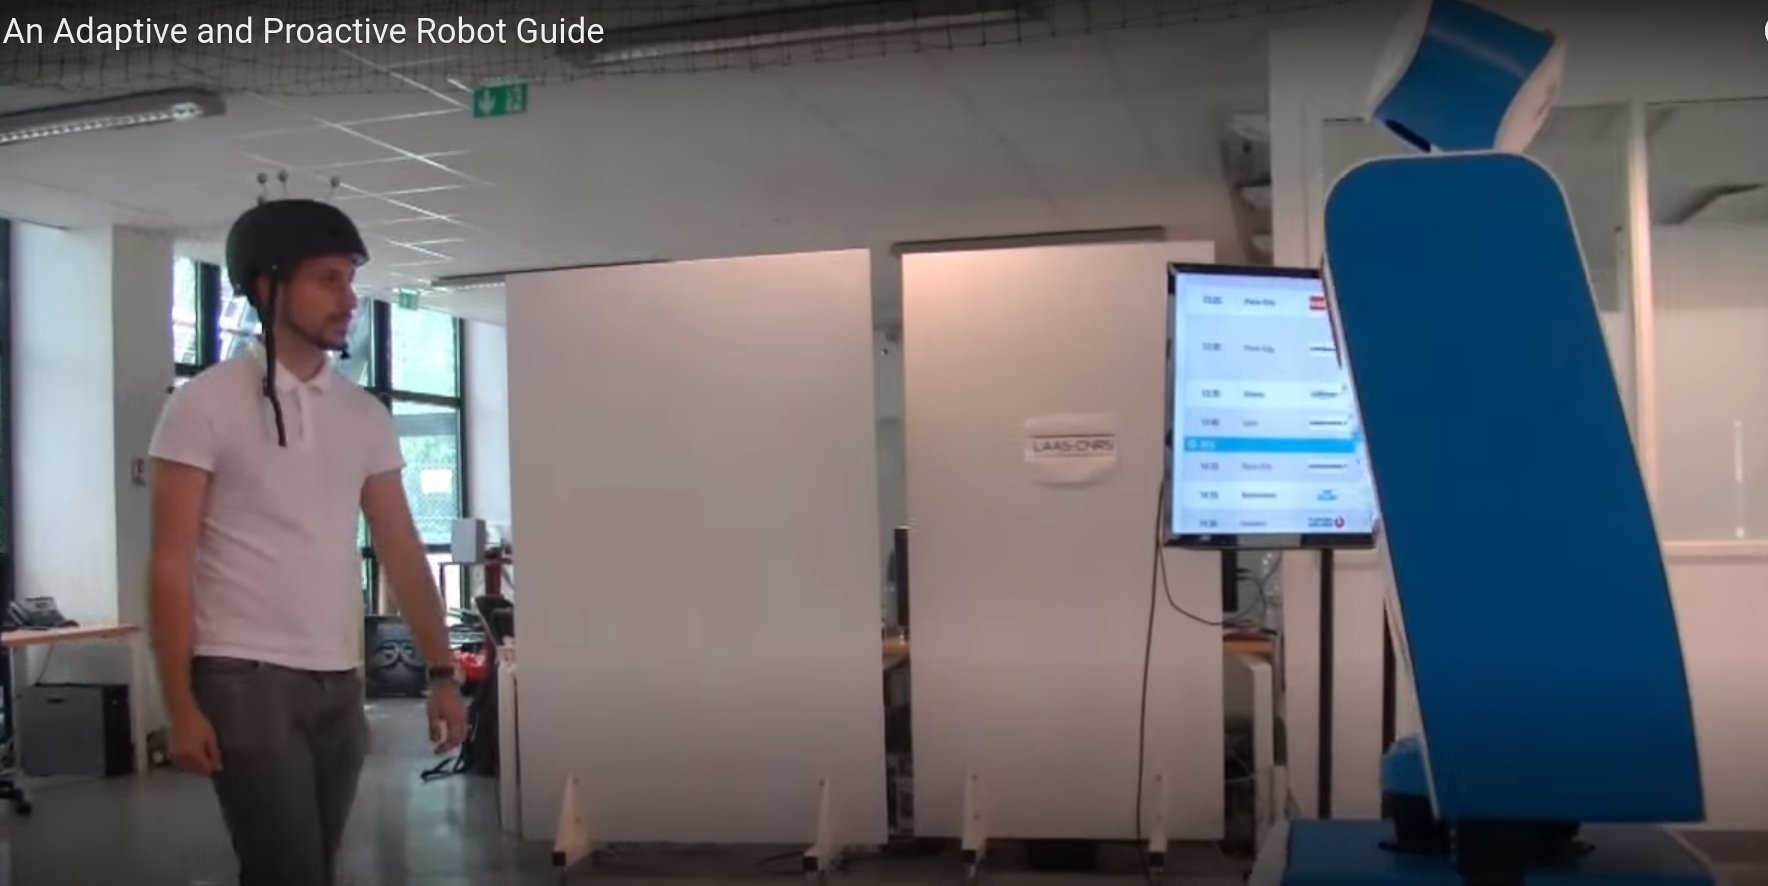
\includegraphics[width=0.68\textwidth]{./img/spenc1.jpg}\label{init}}
    \subfigure[L'homme s'arrête pour consulter un écran d'informations]{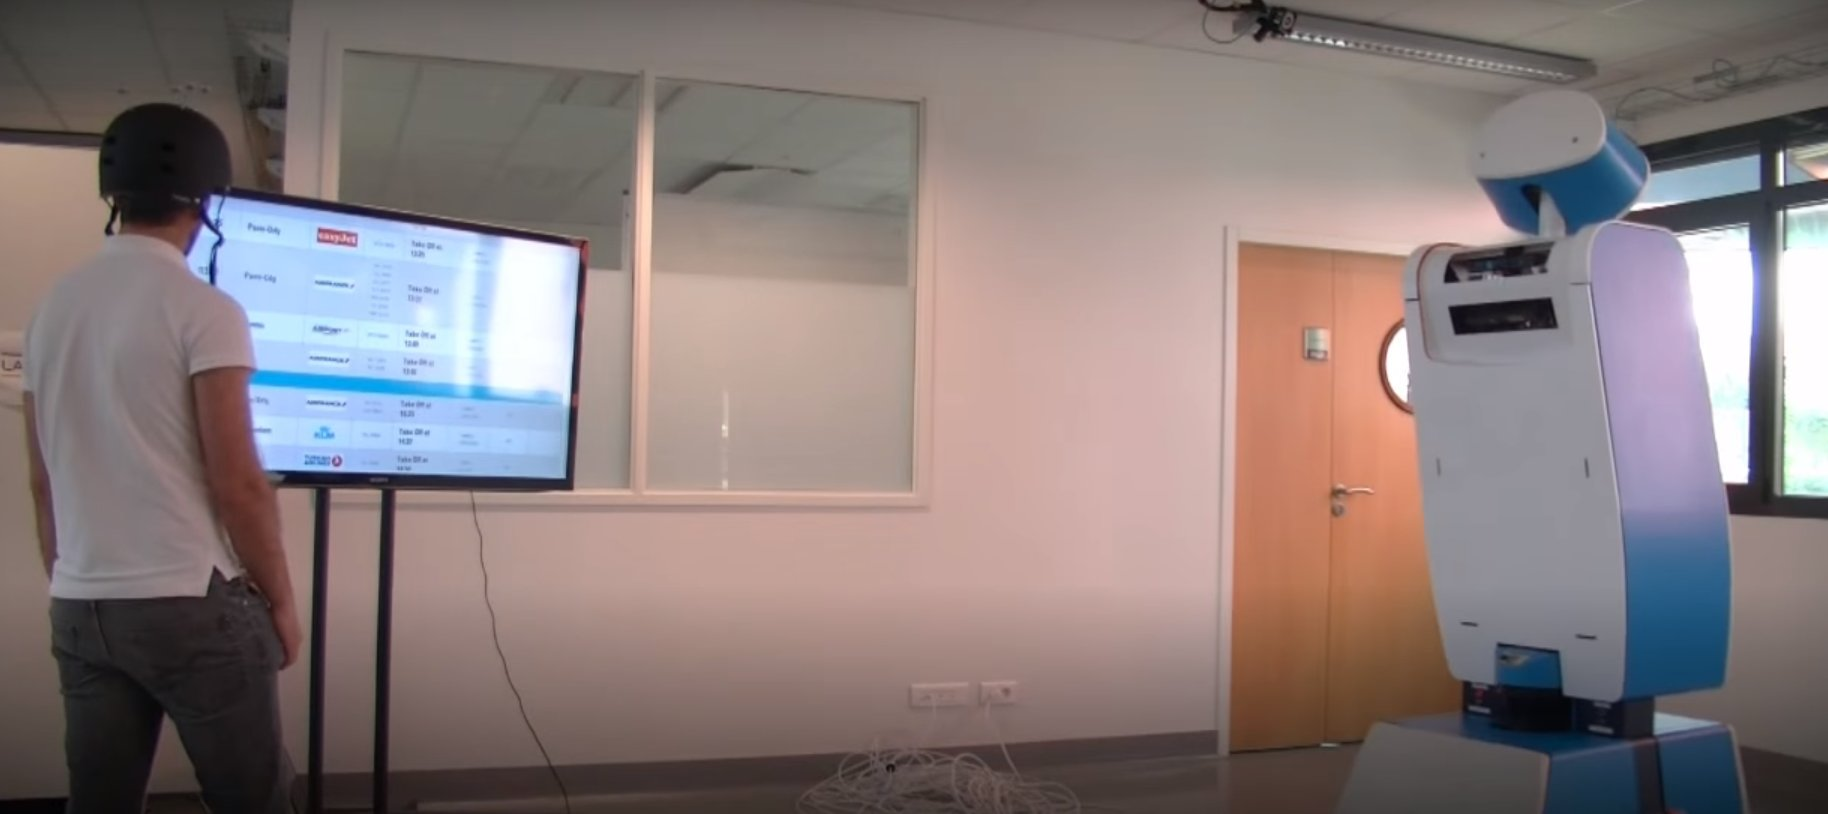
\includegraphics[width=0.68\textwidth]{./img/spenc2.jpg}\label{screen}}
    \subfigure[Le robot donne des informations complémentaire de façon proactive.]{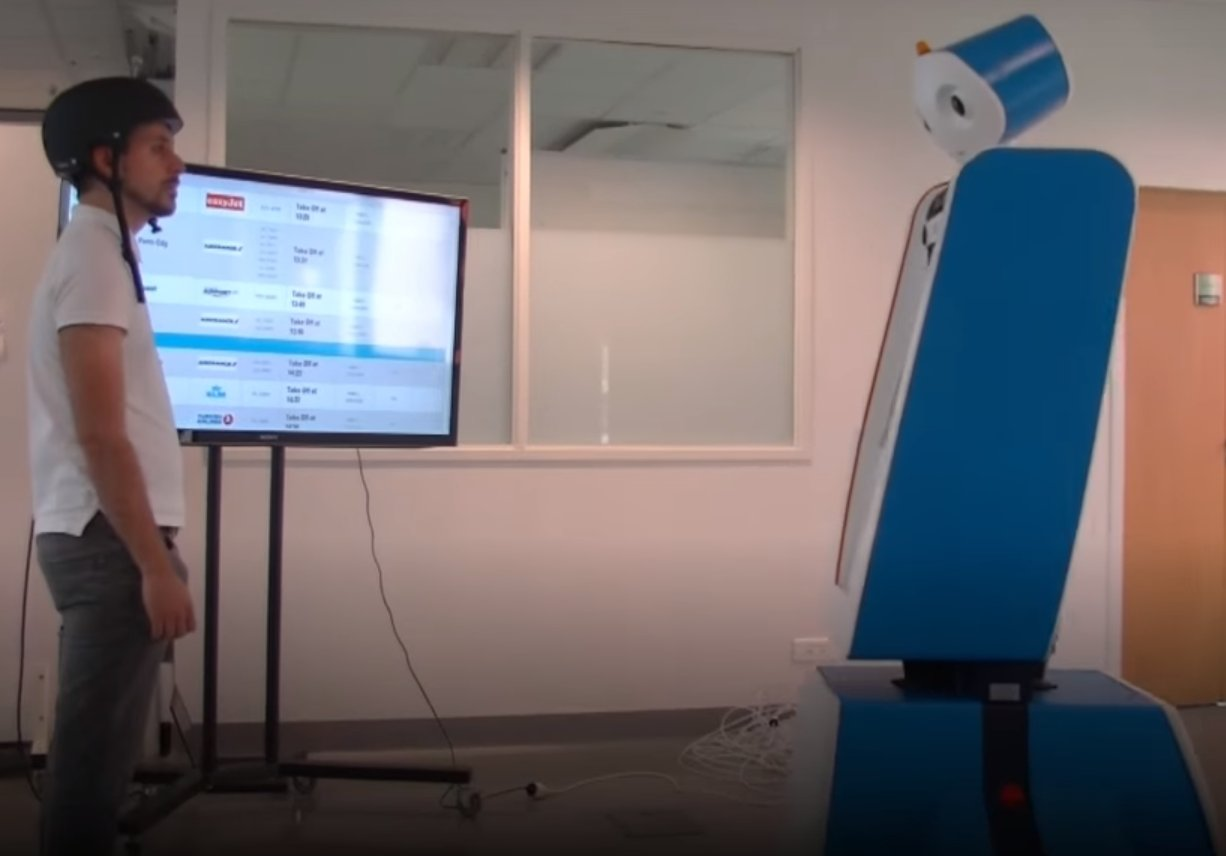
\includegraphics[width=0.55\textwidth]{./img/spencer3.jpg}\label{info}}
 \end{center}
  \caption{Dans cet exemple, le robot qui doit guider l'humain estime que celui-ci est pris dans une tâche secondaire temporaire (ici consulter un écran d'informations). Plutôt que d'abandonner la tâche, le robot décide alors de s'approcher de l'homme pour lui donner des informations complémentaires avant de reprendre la tâche de guide.}
  \label{fig:screen}
\end{figure*}

 
%This situation assessment gives, to the robot, the capacity to detect that one or more of the human followers are involved in a temporary activity. The robot can then disambiguate between situation where it should give up on guiding and situation where it should wait for the humans, or even proactively help the humans involved in the activity.

%TODO: rewrite to adapt to toaster
%To be relevant, reasoning on humans should be linked to the environment. The system is able to create activity areas in the environment and link them to different kind of computations. An activity area is a polygonal or circular area, which can be fixed or linked and updated with an entity's (object, human or robot) position. For now, we studied and experimented different activity areas: a) Information Screen Area, linked to information screens present in the environment; b) Touristic Point Area, linked to interesting attractions in the environment.
%Using these areas, the system can detect human activities (e.g. human is looking at an information screen, human is looking at an attraction).


%
%We believe that to be socially acceptable, the robot should adapt its speed to the group. By setting its own pace at the start of the scenario the robot  would risk of being too slow, annoying the users, or too fast, which would lead the robot to constantly stop to wait for the group, producing an awkward behavior.

%The robot defines a desired range of distance $r$ from the group. The distance of the  members of the group from $r$ will influence its actions. 1) If there is a member of the group farther than $r$ the robot will \textit{decelerate}. The main goal of a guide robot should still be guiding all of the group, and so the robot will give priority to people that would like a slower speed. 2) If 1) is false, and the majority of the group is closer to the robot than $r$, the robot will $accelerate$. 3) If 1) and 2) are false, the robot will continue at its pace.


%In some situation, the robot needs to suspend the task, because the group has stopped following it. In this case, the robot should estimate if this suspension of the collaborative scenario is temporary or permanent, and in the latter case abandon the task. We estimate this information using the Suspend Model and the activity areas from Situation Assessment. We link activity areas to the maximum time we expect that the group will be involved in the linked activity, and with a set of proactive actions that the robot can choose to execute.

%In this paper, we investigated a single possible proactive behavior: giving information. In this case, if we detect that one or more  members
%of the group has stopped following because it is looking at a touristic sight, or at an information screen, the robot can try to engage him and offer related information. At the moment, we just propose a simple routine-based framework for this behavior, and plan to further study it in the future. We believe that the solution of this problem could be rich, and that the robot should estimate the reaction of the group during the execution of its proactive behavior, in order to be able to interrupt if the group doesn't want to be helped or to resume the original task if they are satisfied by the robot's actions.

 \begin{figure}[ht!]
 \centering
 \begin{tabular}{cc}
   \vspace{-5pt}
  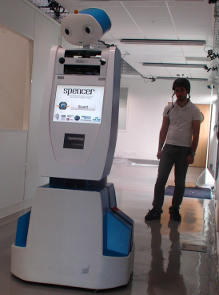
\includegraphics[width=0.4\textwidth]{img/spencer_guidingShrink.png} &
  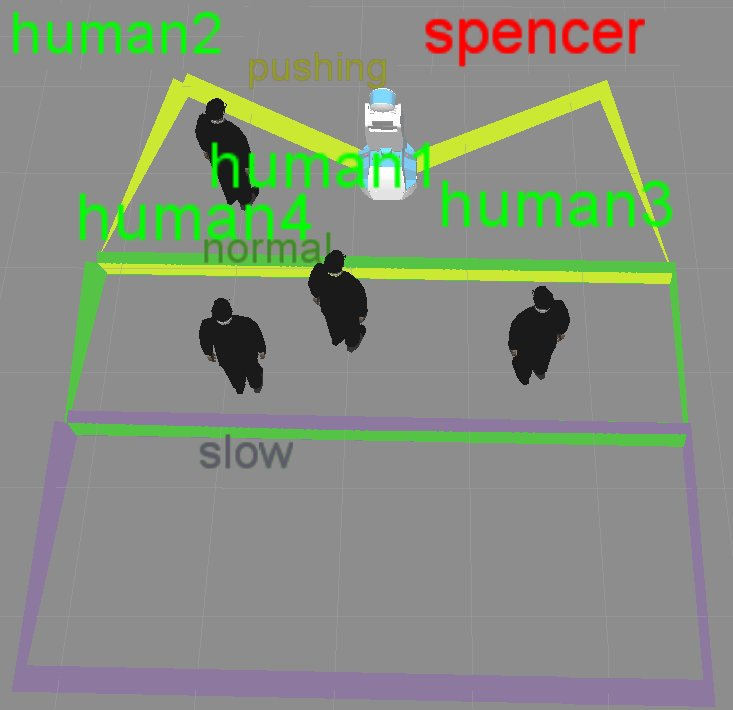
\includegraphics[width=0.56\textwidth]{img/toaster_spencer.jpg}
 \end{tabular}
 \caption{Le robot Spencer, dans le monde réel (à gauche) et dans TOASTER (à droite) avec les zones qui lui sont attachées pour guider les humains.}
 \label{fig:spencer}
  % \vspace{-10pt}
 \end{figure}
 
 
\subsection{Le robot coéquipier}
L'un des autres projets utilisant l'infrastructure logicielle TOASTER visait à construire un robot pour travailler avec un humain sur une chaîne d'assemblage.
Dans ce scénario, le robot partage l'espace de travail avec un humain. Par conséquent, il est essentiel de pouvoir estimer à tout moment la situation spatiale de l'homme et son activité.
Le système se repose sur le module \textit{PDG} de TOASTER pour regrouper les données depuis les capteurs et construire le modèle d'environnement.
Il utilise également le module \textit{SPAR} pour avoir une représentation symbolique de l'état du monde, le module de gestion des zones pour savoir à quelle station de travail l'humain se trouve et le module de suivi des agents pour estimer l'action courante de l'homme.
En utilisant les faits provenant de ces modules, lui procurant une représentation symbolique de l'état du monde et de la situation de l'interaction, le robot est capable d'adapter son comportement à l'humain avec lequel il collabore.
La première façon d'utiliser les informations de TOASTER est d'assurer la sécurité en arrêtant le déplacement du robot lorsque l'homme est dans la même zone de travail et lorsqu'il est en train de se déplacer.
Un autre moyen de s'adapter est de transmettre la représentation symbolique  de l'état du monde (l'ensemble des faits) à un planificateur afin d'aider l'homme de façon proactive. En effet, avec la connaissance de l'état du monde actuel, reliée à la compréhension de l'activité de l'homme, le robot peut estimer l'étape actuelle du plan à accomplir et agir afin d'aider l'homme pour les étapes suivantes du plan. Par exemple, lorsque l'homme est en train de nettoyer une pièce à assembler, si l'étape suivante est de visser cette pièce, le robot peut apporter la visseuse à l'homme. L'image \ref{fig:saphari} illustre la situation où le robot détecte que l'homme tend le bras et est orienté en direction du robot. En utilisant ces faits, le robot suppose que l'homme est prêt à recevoir l'objet et le lui donne.

%Add TOASTER image?

 \begin{figure}[ht!]

 \centering
 \begin{tabular}{cc}
  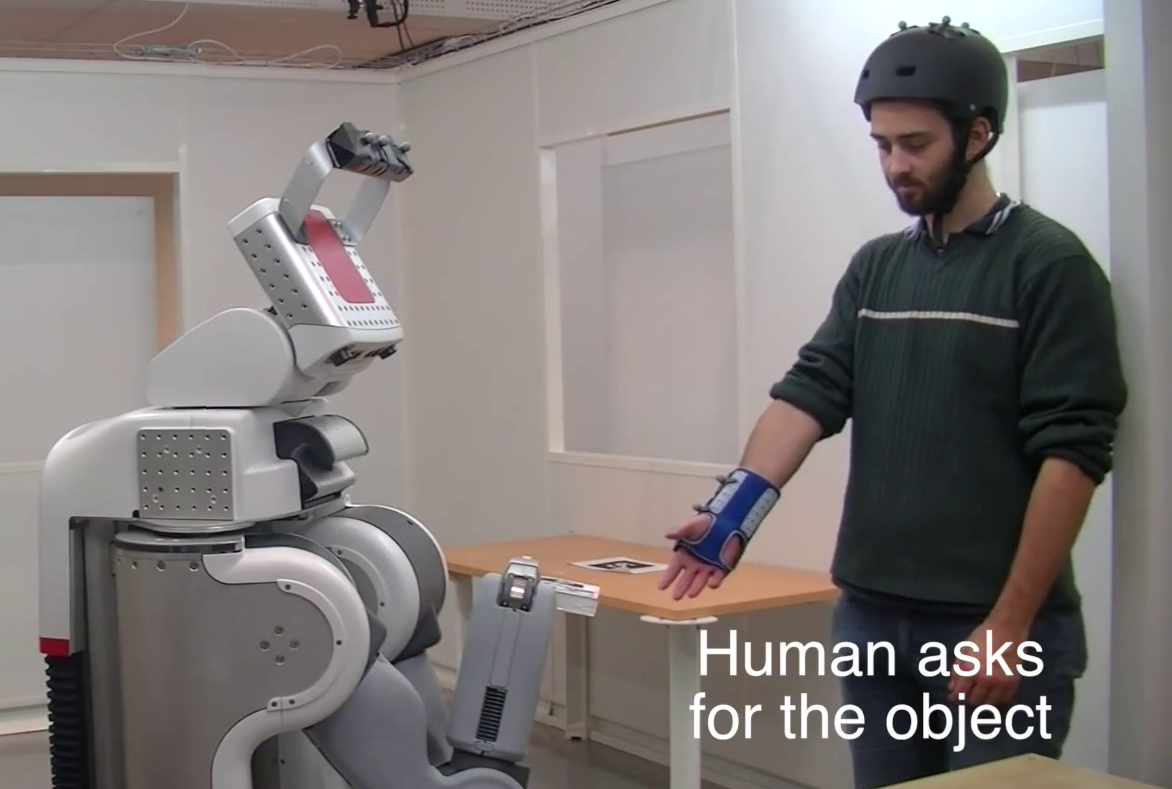
\includegraphics[width=0.7\textwidth]{img/sapharishrink.png}
 \end{tabular}
 \caption{Le robot détecte que l'homme demande l'objet en utilisant la distance de la main par rapport à son corps, grâce au module de suivi d'agent de TOASTER, pour comprendre que l'homme est en train de tendre le bras. Ici, un système de capture de mouvement est utilisé pour suivre les positions de la tête et du bras de l'homme.}
 \label{fig:saphari}
 \end{figure}
 
 
 Ces deux exemples d'utilisation de l'infrastructure logicielle dans deux projets différents illustrent la généricité, la simplicité de configuration grâce à l'architecture modulaire, ainsi que la polyvalence de TOASTER. Dans ces deux projets d'interaction homme robot, les faits produits par TOASTER ont permis de fournir les informations nécessaires à la couche décisionnelle pour pouvoir s'adapter à l'homme et donner un comportement socialement acceptable au robot.

%\section{Gestion de l'Incertitude}
%TODO?
%humain prends un objet dans panier à 2 objets
%-> 50 / 50?
% 
%\section{Bilan}



\ifdefined\included
\else
\bibliographystyle{acm}
\bibliography{These}
\end{document}
\fi